\chapter{Problemas Adicionales: Cálculo de Probabilidades (V. Quesada)}

\section{Sucesiones de conjuntos. Álgebras y \texorpdfstring{$\sigma$}{sigma}-álgebras}

% ------------------------------------------------------------------------------
% PROBLEMA 1
% ------------------------------------------------------------------------------
\begin{problema}[Límite de sucesiones de intervalos]
Dadas las siguientes sucesiones de subconjuntos de $\mathbb{R}$:
\begin{enumerate}[label=\alph*)]
    \item $A_n = \left\{ x \in \mathbb{R} \,\,\middle|\,\, \frac{1}{n} \le x \le 3 - \frac{1}{n} \right\}$
    \item $A_n = \left\{ x \in \mathbb{R} \,\,\middle|\,\, 2 < x \le 2 + \frac{1}{n} \right\}$
\end{enumerate}
Encontrar $\displaystyle \lim_{n \to \infty} A_n$ en cada caso.

\tcblower

\begin{enumerate}[label=\alph*)]
    \item \textbf{Análisis de la sucesión $A_n = \left[\frac{1}{n}, 3 - \frac{1}{n}\right]$:}
    
    Evaluamos los primeros términos de la sucesión para determinar su comportamiento:
    \[
        A_1 = [1, 2], \quad A_2 = \left[\frac{1}{2}, \frac{5}{2}\right], \quad A_3 = \left[\frac{1}{3}, \frac{8}{3}\right], \quad \dots
    \]
    La sucesión es monótona creciente, ya que $A_n \subseteq A_{n+1}$ para todo $n \in \mathbb{N}$. Por tanto, la sucesión es convergente y su límite coincide con la unión infinita de sus términos:
    \[
        \lim_{n \to \infty} A_n = \bigcup_{n=1}^\infty A_n = (0, 3)
    \]
    
    \textit{Justificación de los extremos del intervalo:}
    \begin{itemize}
        \item Extremo inferior ($0$): Para cualquier $x > 0$, existe $n_0 \in \mathbb{N}$ tal que $\frac{1}{n_0} < x$, de modo que $x \in A_{n_0} \subseteq \bigcup A_n$. Sin embargo, el $0$ no pertenece a ningún $A_n$ puesto que $\frac{1}{n} > 0$ para todo $n \in \mathbb{N}$.
        \item Extremo superior ($3$): Para cualquier $x < 3$, existe $n_0 \in \mathbb{N}$ tal que $x < 3 - \frac{1}{n_0}$, por lo que $x \in A_{n_0} \subseteq \bigcup A_n$. Sin embargo, el $3$ no pertenece a ningún $A_n$ dado que $3 - \frac{1}{n} < 3$ para todo $n \in \mathbb{N}$.
    \end{itemize}

    \item \textbf{Análisis de la sucesión $A_n = \left(2, 2 + \frac{1}{n}\right]$:}
    
    Evaluamos los primeros términos:
    \[
        A_1 = (2, 3], \quad A_2 = \left(2, \frac{5}{2}\right], \quad A_3 = \left(2, \frac{7}{3}\right], \quad \dots
    \]
    La sucesión es monótona decreciente, ya que $A_n \supseteq A_{n+1}$ para todo $n \in \mathbb{N}$. Por lo tanto, la sucesión es convergente y su límite es la intersección infinita de sus términos:
    \[
        \lim_{n \to \infty} A_n = \bigcap_{n=1}^\infty A_n = \varnothing
    \]
    
    \textit{Justificación:} Si existiera un elemento $x \in \bigcap_{n=1}^\infty A_n$, se tendría $x > 2$ y $x \le 2 + \frac{1}{n}$ para todo $n \in \mathbb{N}$. Tomando el límite cuando $n \to \infty$, resultaría $x \le 2$, lo cual contradice $x > 2$. Por consiguiente, la intersección es vacía.
\end{enumerate}
\end{problema}
\newpage
% ------------------------------------------------------------------------------
% PROBLEMA 2
% ------------------------------------------------------------------------------
\begin{problema}[Leyes de De Morgan para límites de conjuntos]
Sea $\{A_n\}_{n \in \mathbb{N}}$ una sucesión arbitraria de subconjuntos de $\Omega$. Demostrar que:
\begin{enumerate}[label=\alph*)]
    \item $\displaystyle \varlimsup_{n \to \infty} A_n^c = \left( \varliminf_{n \to \infty} A_n \right)^c$
    \item $\displaystyle \varliminf_{n \to \infty} A_n^c = \left( \varlimsup_{n \to \infty} A_n \right)^c$
\end{enumerate}

\tcblower

Utilizamos la caracterización de los límites superior e inferior mediante uniones e intersecciones infinitas y aplicamos las leyes de De Morgan generalizadas:

\begin{enumerate}[label=\alph*)]
    \item \textbf{Demostración de $\displaystyle \varlimsup_{n \to \infty} A_n^c = \left( \varliminf_{n \to \infty} A_n \right)^c$:}
    
    Expresamos la definición del límite superior sobre los complementarios $A_n^c$:
    \[
        \varlimsup_{n \to \infty} A_n^c = \bigcap_{n=1}^\infty \bigcup_{j=n}^\infty A_j^c
    \]
    Aplicando De Morgan a la unión de la cola, $\bigcup_{j=n}^\infty A_j^c = \left( \bigcap_{j=n}^\infty A_j \right)^c$:
    \[
        \varlimsup_{n \to \infty} A_n^c = \bigcap_{n=1}^\infty \left( \bigcap_{j=n}^\infty A_j \right)^c
    \]
    Aplicando De Morgan a la intersección infinita exterior:
    \[
        \bigcap_{n=1}^\infty \left( \bigcap_{j=n}^\infty A_j \right)^c = \left( \bigcup_{n=1}^\infty \bigcap_{j=n}^\infty A_j \right)^c
    \]
    Como la expresión entre paréntesis es la caracterización del límite inferior, $\displaystyle \varliminf_{n \to \infty} A_n = \bigcup_{n=1}^\infty \bigcap_{j=n}^\infty A_j$, concluimos:
    \[
        \varlimsup_{n \to \infty} A_n^c = \left( \varliminf_{n \to \infty} A_n \right)^c
    \]

    \item \textbf{Demostración de $\displaystyle \varliminf_{n \to \infty} A_n^c = \left( \varlimsup_{n \to \infty} A_n \right)^c$:}
    
    Expresamos el límite inferior de la sucesión de complementarios $A_n^c$:
    \[
        \varliminf_{n \to \infty} A_n^c = \bigcup_{n=1}^\infty \bigcap_{j=n}^\infty A_j^c
    \]
    Aplicando De Morgan a la intersección de la cola, $\bigcap_{j=n}^\infty A_j^c = \left( \bigcup_{j=n}^\infty A_j \right)^c$:
    \[
        \varliminf_{n \to \infty} A_n^c = \bigcup_{n=1}^\infty \left( \bigcup_{j=n}^\infty A_j \right)^c
    \]
    Aplicando De Morgan a la unión infinita exterior:
    \[
        \bigcup_{n=1}^\infty \left( \bigcup_{j=n}^\infty A_j \right)^c = \left( \bigcap_{n=1}^\infty \bigcup_{j=n}^\infty A_j \right)^c
    \]
    Como la expresión entre paréntesis es la caracterización del límite superior, $\displaystyle \varlimsup_{n \to \infty} A_n = \bigcap_{n=1}^\infty \bigcup_{j=n}^\infty A_j$, concluimos:
    \[
        \varliminf_{n \to \infty} A_n^c = \left( \varlimsup_{n \to \infty} A_n \right)^c
    \]
\end{enumerate}
\end{problema}
\newpage
% ------------------------------------------------------------------------------
% PROBLEMA 3
% ------------------------------------------------------------------------------
\begin{problema}[Límites superior e inferior de subsucesiones pares e impares]
Sea $\{A_n\}_{n \in \mathbb{N}}$ una sucesión arbitraria de subconjuntos de $\Omega$. Estudiar la relación entre los límites superior e inferior de la sucesión $\{A_n\}$ y los de sus subsucesiones de términos pares $\{A_{2n}\}$ e impares $\{A_{2n-1}\}$.

\tcblower

\begin{enumerate}[label=\alph*)]
    \item \textbf{Relación para el límite superior:}
    
    Un elemento $x \in \Omega$ pertenece al límite superior $\varlimsup_{n \to \infty} A_n$ si y solo si pertenece a infinitos términos de la sucesión $\{A_n\}$. Como todo término $A_n$ tiene índice par o impar, estar en infinitos conjuntos de $\{A_n\}$ equivale a estar en infinitos conjuntos de la subsucesión $\{A_{2n}\}$ o bien en infinitos conjuntos de la subsucesión $\{A_{2n-1}\}$.
    
    Formalmente:
    \begin{align*}
        x \in \varlimsup_{n \to \infty} A_n &\iff x \in A_n \text{ para infinitos subíndices } n \in \mathbb{N} \\
        &\iff x \in \varlimsup_{n \to \infty} A_{2n} \quad \text{o} \quad x \in \varlimsup_{n \to \infty} A_{2n-1} \\
        &\iff x \in \left( \varlimsup_{n \to \infty} A_{2n} \cup \varlimsup_{n \to \infty} A_{2n-1} \right)
    \end{align*}
    Por tanto, se verifica la igualdad:
    \[
        \varlimsup_{n \to \infty} A_n = \varlimsup_{n \to \infty} A_{2n} \cup \varlimsup_{n \to \infty} A_{2n-1}
    \]

    \item \textbf{Relación para el límite inferior:}
    
    Un elemento $x \in \Omega$ pertenece al límite inferior $\varliminf_{n \to \infty} A_n$ si y solo si pertenece a todos los términos de la sucesión $\{A_n\}$ salvo a un número finito de ellos. Esto exige que pertenezca a todos los términos pares salvo a un número finito, y simultáneamente a todos los términos impares salvo a un número finito.
    
    Formalmente:
    \begin{align*}
        x \in \varliminf_{n \to \infty} A_n &\iff x \in A_n \text{ para todo } n \in \mathbb{N} \text{ salvo un número finito} \\
        &\iff x \in \varliminf_{n \to \infty} A_{2n} \quad \text{y} \quad x \in \varliminf_{n \to \infty} A_{2n-1} \\
        &\iff x \in \left( \varliminf_{n \to \infty} A_{2n} \cap \varliminf_{n \to \infty} A_{2n-1} \right)
    \end{align*}
    Por tanto, se verifica la igualdad:
    \[
        \varliminf_{n \to \infty} A_n = \varliminf_{n \to \infty} A_{2n} \cap \varliminf_{n \to \infty} A_{2n-1}
    \]
\end{enumerate}
\end{problema}
\newpage

% ------------------------------------------------------------------------------
% PROBLEMA 4
% ------------------------------------------------------------------------------
\begin{problema}[Cálculo del límite de una sucesión alternante de intervalos]
Sea $\{E_n\}_{n \in \mathbb{N}}$ la sucesión de subconjuntos de $\mathbb{R}$ definida por:
\[
    E_{2n-1} = \left\{ x \in \mathbb{R} \,\,\middle|\,\, 0 < x \le 1 - \frac{1}{2n-1} \right\} \quad \text{y} \quad E_{2n} = \left\{ x \in \mathbb{R} \,\,\middle|\,\, \frac{1}{2n} \le x < 1 \right\}
\]
Calcular, si existe, $\displaystyle \lim_{n \to \infty} E_n$.

\tcblower

Utilizando las identidades obtenidas en el Problema 3, podemos descomponer los límites superior e inferior de la sucesión $\{E_n\}$ mediante sus subsucesiones de términos impares $\{E_{2n-1}\}$ y pares $\{E_{2n}\}$:
\[
    \varlimsup_{n \to \infty} E_n = \varlimsup_{n \to \infty} E_{2n} \cup \varlimsup_{n \to \infty} E_{2n-1} \quad \text{y} \quad \varliminf_{n \to \infty} E_n = \varliminf_{n \to \infty} E_{2n} \cap \varliminf_{n \to \infty} E_{2n-1}
\]

Analizamos el comportamiento de cada subsucesión:

\begin{enumerate}[label=\arabic*.]
    \item \textbf{Subsucesión impar $E_{2n-1} = \left(0, 1 - \frac{1}{2n-1}\right]$:}
    
    Como $1 - \frac{1}{2n-1}$ crece estrictamente hacia $1$ cuando $n \to \infty$, la sucesión de conjuntos $\{E_{2n-1}\}$ es monótona creciente ($E_{2n-1} \subseteq E_{2n+1}$). Por consiguiente, es convergente y su límite viene dado por la unión numerable:
    \[
        \lim_{n \to \infty} E_{2n-1} = \bigcup_{n=1}^\infty \left(0, 1 - \frac{1}{2n-1}\right] = (0, 1)
    \]
    Así pues:
    \[
        \varlimsup_{n \to \infty} E_{2n-1} = \varliminf_{n \to \infty} E_{2n-1} = (0, 1)
    \]

    \item \textbf{Subsucesión par $E_{2n} = \left[\frac{1}{2n}, 1\right)$:}
    
    Como $\frac{1}{2n}$ decrece estrictamente hacia $0$ cuando $n \to \infty$, el extremo inferior del intervalo se expande hacia la izquierda, por lo que la sucesión $\{E_{2n}\}$ es también monótona creciente ($E_{2n} \subseteq E_{2n+2}$). Por consiguiente, es convergente y su límite es:
    \[
        \lim_{n \to \infty} E_{2n} = \bigcup_{n=1}^\infty \left[\frac{1}{2n}, 1\right) = (0, 1)
    \]
    Así pues:
    \[
        \varlimsup_{n \to \infty} E_{2n} = \varliminf_{n \to \infty} E_{2n} = (0, 1)
    \]
\end{enumerate}

Sustituyendo los resultados en las relaciones de límites superior e inferior:
\[
    \varlimsup_{n \to \infty} E_n = (0, 1) \cup (0, 1) = (0, 1)
\]
\[
    \varliminf_{n \to \infty} E_n = (0, 1) \cap (0, 1) = (0, 1)
\]

Al coincidir ambos límites, la sucesión $\{E_n\}$ es convergente y su límite es:
\[
    \lim_{n \to \infty} E_n = (0, 1)
\]
\end{problema}
\newpage
% ------------------------------------------------------------------------------
% PROBLEMA 5
% ------------------------------------------------------------------------------
\begin{problema}[Límite de regiones circulares en $\mathbb{R}^2$]
Dadas las siguientes sucesiones de subconjuntos de $\mathbb{R}^2$:
\begin{enumerate}[label=\alph*)]
    \item $A_n = \left\{ (x,y) \in \mathbb{R}^2 \,\,\middle|\,\, \frac{1}{n} \le x^2 + y^2 \le 4 - \frac{1}{n} \right\}$
    \item $A_n = \left\{ (x,y) \in \mathbb{R}^2 \,\,\middle|\,\, 0 \le x^2 + y^2 \le \frac{1}{n} \right\}$
\end{enumerate}
Encontrar $\displaystyle \lim_{n \to \infty} A_n$ en cada caso.

\tcblower

\begin{enumerate}[label=\alph*)]
    \item \textbf{Análisis de la sucesión de coronas circulares $A_n$:}
    
    Observamos la relación de inclusión entre términos consecutivos:
    \[
        \frac{1}{n+1} < \frac{1}{n} \quad \text{y} \quad 4 - \frac{1}{n} < 4 - \frac{1}{n+1}
    \]
    Esto implica que los anillos se van expandiendo tanto interior como exteriormente, de modo que $A_n \subseteq A_{n+1}$ para todo $n \in \mathbb{N}$. La sucesión es monótona creciente y, por tanto, convergente. Su límite coincide con la unión infinita de sus términos:
    \[
        \lim_{n \to \infty} A_n = \bigcup_{n=1}^\infty A_n = \left\{ (x,y) \in \mathbb{R}^2 \,\,\middle|\,\, 0 < x^2 + y^2 < 4 \right\}
    \]
    Geométricamente, el límite corresponde a la bola abierta de radio $2$ centrada en el origen excluyendo el origen $(0,0)$.

    \item \textbf{Análisis de la sucesión de discos $A_n$:}
    
    Dado que $\frac{1}{n+1} < \frac{1}{n}$, el radio de los discos decrece estrictamente a medida que $n$ aumenta, verificándose que $A_{n+1} \subseteq A_n$ para todo $n \in \mathbb{N}$. La sucesión es monótona decreciente y, por tanto, convergente. Su límite es la intersección infinita de sus términos:
    \[
        \lim_{n \to \infty} A_n = \bigcap_{n=1}^\infty A_n = \left\{ (x,y) \in \mathbb{R}^2 \,\,\middle|\,\, x^2 + y^2 = 0 \right\} = \{(0,0)\}
    \]
    El límite es el conjunto unipuntual formado exclusivamente por el origen de coordenadas.
\end{enumerate}
\end{problema}
\newpage
% ------------------------------------------------------------------------------
% PROBLEMA 6
% ------------------------------------------------------------------------------
\begin{problema}[Convergencia de sucesiones mediante diferencia simétrica]
Sea $\{E_n\}_{n \in \mathbb{N}}$ una sucesión de subconjuntos de $\Omega$. Se construye la sucesión $\{D_n\}_{n \in \mathbb{N}}$ del siguiente modo:
\[
    D_1 = E_1, \quad D_2 = D_1 \Delta E_2, \quad \dots, \quad D_n = D_{n-1} \Delta E_n, \quad \dots
\]
donde $\Delta$ representa la diferencia simétrica. Demostrar que $\{D_n\}_{n \in \mathbb{N}}$ es convergente si y solo si $\displaystyle \lim_{n \to \infty} E_n = \varnothing$.

\tcblower

\textit{Propiedad clave previa:} Puesto que la diferencia simétrica satisface $A \Delta B = C \iff A \Delta C = B$, de la relación recurrente $D_n = D_{n-1} \Delta E_n$ se deduce directamente que:
\[
    E_n = D_{n-1} \Delta D_n = (D_{n-1} \setminus D_n) \cup (D_n \setminus D_{n-1})
\]

Demostramos la equivalencia en dos pasos:

\begin{enumerate}
    \item \textbf{Implicación $(\impliedby)$:} Supongamos que $\displaystyle \lim_{n \to \infty} E_n = \varnothing$.
    
    Esto significa que $\varlimsup_{n \to \infty} E_n = \varnothing$, por lo que todo elemento $x \in \Omega$ pertenece únicamente a un número finito de conjuntos de la sucesión $\{E_n\}$.
    
    Dado un $x \in \Omega$ arbitrario, existe un índice $k \in \mathbb{N}$ tal que $x \notin E_n$ para todo $n \ge k$. Analizamos el comportamiento de $D_n$ para $n \ge k$:
    \[
        D_n = D_{n-1} \Delta E_n = (D_{n-1} \setminus E_n) \cup (E_n \setminus D_{n-1})
    \]
    Como $x \notin E_n$, la condición de pertenencia $x \in D_n$ equivale exactamente a $x \in D_{n-1}$. Por inducción, la pertenencia de $x$ a $D_n$ se vuelve constante para todo $n \ge k-1$:
    \begin{itemize}
        \item Si $x \in D_{k-1}$, entonces $x \in D_n$ para todo $n \ge k-1$, de donde $x \in \varliminf_{n \to \infty} D_n$.
        \item Si $x \notin D_{k-1}$, entonces $x \notin D_n$ para todo $n \ge k-1$, de donde $x \notin \varlimsup_{n \to \infty} D_n$.
    \end{itemize}
    En cualquier caso, se verifica que $\varlimsup_{n \to \infty} D_n = \varliminf_{n \to \infty} D_n$, lo que prueba que $\{D_n\}$ es convergente.

    \item \textbf{Implicación $(\implies)$:} Supongamos que $\{D_n\}$ es una sucesión convergente, es decir, existe el límite $D = \lim_{n \to \infty} D_n = \varlimsup_{n \to \infty} D_n = \varliminf_{n \to \infty} D_n$.
    
    Dado un elemento cualquiera $x \in \Omega$, distinguimos los dos únicos casos posibles:
    \begin{itemize}
        \item \textit{Caso 1 ($x \in D$):} Puesto que $x \in \varliminf_{n \to \infty} D_n$, existe un $N_1 \in \mathbb{N}$ tal que $x \in D_n$ para todo $n \ge N_1$. En particular, para todo $n > N_1$ se cumple $x \in D_{n-1}$ y $x \in D_n$. Por la propiedad clave, $E_n = D_{n-1} \Delta D_n$, luego $x \notin E_n$ para todo $n > N_1$.
        \item \textit{Caso 2 ($x \notin D$):} Puesto que $x \notin \varlimsup_{n \to \infty} D_n$, existe un $N_2 \in \mathbb{N}$ tal que $x \notin D_n$ para todo $n \ge N_2$. En particular, para todo $n > N_2$ se cumple $x \notin D_{n-1}$ y $x \notin D_n$, luego $x \notin E_n$ para todo $n > N_2$.
    \end{itemize}
    En ambos casos, todo elemento $x \in \Omega$ pertenece como máximo a un número finito de conjuntos $E_n$. Por tanto, $x \notin \varlimsup_{n \to \infty} E_n$, de lo que se concluye que $\varlimsup_{n \to \infty} E_n = \varnothing$ y, por ende:
    \[
        \lim_{n \to \infty} E_n = \varnothing
    \]
\end{enumerate}
\end{problema}

\newpage
% ------------------------------------------------------------------------------
% PROBLEMA 7
% ------------------------------------------------------------------------------
\begin{problema}[$\sigma$-álgebra de subconjuntos invariantes por una biyección]
Sea $\Omega$ un conjunto universal arbitrario y $f : \Omega \to \Omega$ una aplicación biyectiva. Se define la clase de subconjuntos de $\Omega$ invariantes por $f$ como:
\[
    \mathcal{S} = \{ A \in \mathcal{P}(\Omega) \mid f(A) = A \}
\]
donde $f(A) = \{ f(\omega) \in \Omega \mid \omega \in A \}$. Demostrar que $\mathcal{S}$ tiene estructura de $\sigma$-álgebra sobre $\Omega$.

\tcblower

Comprobamos que la clase $\mathcal{S}$ satisface los tres axiomas fundamentales de $\sigma$-álgebra:

\begin{enumerate}
    \item \textbf{Pertenencia del conjunto universal:}
    
    Como la aplicación $f : \Omega \to \Omega$ es biyectiva, en particular es suprayectiva (epiyectiva), por lo que la imagen directa del espacio completo satisface $f(\Omega) = \Omega$. Por consiguiente:
    \[
        \Omega \in \mathcal{S}
    \]

    \item \textbf{Cierre por complementación:}
    
    Sea $A \in \mathcal{S}$, lo que significa que $f(A) = A$. Analizamos la imagen del complementario $A^c = \Omega \setminus A$.
    
    Puesto que $f$ es una biyección, para cualquier par de conjuntos se cumple $f(\Omega \setminus A) = f(\Omega) \setminus f(A)$. Aplicando la propiedad de invariancia de $A$ y la suprayectividad sobre $\Omega$:
    \[
        f(A^c) = f(\Omega \setminus A) = f(\Omega) \setminus f(A) = \Omega \setminus A = A^c
    \]
    Dado que $f(A^c) = A^c$, se concluye que:
    \[
        A^c \in \mathcal{S}
    \]

    \item \textbf{Cierre por uniones numerables:}
    
    Sea $\{A_n\}_{n \in \mathbb{N}} \subseteq \mathcal{S}$ una sucesión numerable de conjuntos invariantes, es decir, $f(A_n) = A_n$ para todo $n \in \mathbb{N}$.
    
    Aprovechando la propiedad de la imagen directa de conmuta con la unión numerables arbitraria (propiedad que se verifica para cualquier aplicación $f$):
    \[
        f\left( \bigcup_{n=1}^\infty A_n \right) = \bigcup_{n=1}^\infty f(A_n) = \bigcup_{n=1}^\infty A_n
    \]
    Por tanto, la unión numerable $\bigcup_{n=1}^\infty A_n$ es invariante por $f$, lo que demuestra que:
    \[
        \bigcup_{n=1}^\infty A_n \in \mathcal{S}
    \]
\end{enumerate}

Al verificarse los tres axiomas, queda demostrado que la clase $\mathcal{S}$ es una $\sigma$-álgebra sobre $\Omega$.
\end{problema}
\newpage
% ------------------------------------------------------------------------------
% PROBLEMA 8
% ------------------------------------------------------------------------------
\begin{problema}[$\sigma$-álgebra generada por intervalos semiabiertos en $\mathbb{Q}$]
Sea $\mathbb{Q}$ el conjunto de los números racionales y consideremos la clase de intervalos semiabiertos por la izquierda restringidos a $\mathbb{Q}$:
\[
    \mathcal{C} = \bigl\{ (a, b] \cap \mathbb{Q} \mid a, b \in \mathbb{Q}, \, a < b \bigr\}
\]
Demostrar que la $\sigma$-álgebra generada por $\mathcal{C}$ sobre el espacio universal $\mathbb{Q}$ coincide con el conjunto de sus partes, es decir:
\[
    \sigma(\mathcal{C}) = \mathcal{P}(\mathbb{Q})
\]

\tcblower

Demostramos la igualdad de clases $\sigma(\mathcal{C}) = \mathcal{P}(\mathbb{Q})$ mediante la doble inclusión:

\begin{enumerate}
    \item \textbf{Inclusión $\sigma(\mathcal{C}) \subseteq \mathcal{P}(\mathbb{Q})$:}
    
    Por definición, todos los elementos de la clase generadora $\mathcal{C}$ son subconjuntos de $\mathbb{Q}$, de modo que $\mathcal{C} \subseteq \mathcal{P}(\mathbb{Q})$. 
    
    Dado que el conjunto de partes $\mathcal{P}(\mathbb{Q})$ constituye la $\sigma$-álgebra máxima sobre $\mathbb{Q}$ y $\sigma(\mathcal{C})$ es por definición la menor $\sigma$-álgebra que contiene a $\mathcal{C}$, resulta directamente:
    \[
        \sigma(\mathcal{C}) \subseteq \sigma(\mathcal{P}(\mathbb{Q})) = \mathcal{P}(\mathbb{Q})
    \]

    \item \textbf{Inclusión $\mathcal{P}(\mathbb{Q}) \subseteq \sigma(\mathcal{C})$:}
    
    Sea $x \in \mathbb{Q}$ un número racional arbitrario. Para cada índice $n \in \mathbb{N}$, el intervalo semiabierto $\left(x - \frac{1}{n}, x\right] \cap \mathbb{Q}$ pertenece a la clase generadora $\mathcal{C} \subseteq \sigma(\mathcal{C})$.
    
    Podemos expresar el conjunto unipuntual $\{x\}$ como la intersección numerable decreciente de dichos intervalos:
    \[
        \{x\} = \bigcap_{n=1}^\infty \left( \left(x - \frac{1}{n}, x\right] \cap \mathbb{Q} \right)
    \]
    Al ser $\sigma(\mathcal{C})$ una $\sigma$-álgebra, es cerrada bajo intersecciones numerables. Por consiguiente, todo conjunto unipuntual satisface $\{x\} \in \sigma(\mathcal{C})$ para cualquier $x \in \mathbb{Q}$.

    Sea ahora $A \in \mathcal{P}(\mathbb{Q})$ un subconjunto arbitrario de racionales. Dado que el conjunto de los números racionales $\mathbb{Q}$ es numerable, su subconjunto $A$ es a lo sumo numerable, pudiendo representarse como la unión numerable disjunta de sus elementos individuales:
    \[
        A = \bigcup_{x \in A} \{x\}
    \]
    Puesto que $\{x\} \in \sigma(\mathcal{C})$ para todo $x \in A$ y $\sigma(\mathcal{C})$ es cerrada por uniones numerables, se deduce que $A \in \sigma(\mathcal{C})$.
    
    Como esto se verifica para todo subconjunto de $\mathbb{Q}$, concluimos que:
    \[
        \mathcal{P}(\mathbb{Q}) \subseteq \sigma(\mathcal{C})
    \]
\end{enumerate}

De la combinación de ambas inclusiones se obtiene formalmente la igualdad $\sigma(\mathcal{C}) = \mathcal{P}(\mathbb{Q})$.
\end{problema}
\newpage
% ------------------------------------------------------------------------------
% PROBLEMA 9
% ------------------------------------------------------------------------------
\begin{problema}[Álgebra generada por semirrectas origen en el semieje real]
En el espacio universal $\Omega = [0,\infty)$, se consideran las siguientes clases de subconjuntos:
\begin{enumerate}[label=\alph*)]
    \item Sea $\mathcal{C}_1$ la clase de todos los intervalos de la forma $[0,a)$, donde $a \in \Omega$ o $a = +\infty$. Demostrar que $\mathcal{C}_1$ no es un álgebra.
    \item Sea $\mathcal{C}_2$ la clase de todas las uniones finitas de intervalos de la forma $[a,b)$, donde $a \in \Omega$ y $b \in \Omega$ o $b = +\infty$. Demostrar que $\mathcal{C}_2$ es un álgebra, pero no una $\sigma$-álgebra.
    \item Demostrar que $\mathcal{C}_2 = \mathcal{Q}(\mathcal{C}_1)$.
\end{enumerate}

\tcblower

\begin{enumerate}[label=\alph*)]
    \item \textbf{Estudio de la clase $\mathcal{C}_1$:}
    
    Para cualquier elemento $[0,a) \in \mathcal{C}_1$ con $a \in (0,\infty)$, su complementario relativo a $\Omega = [0,\infty)$ es:
    \[
        [0,a)^c = \Omega \setminus [0,a) = [a,\infty)
    \]
    Para cualquier $a > 0$, el conjunto $[a,\infty)$ no comienza en el origen $0$, por lo que no puede expresarse de la forma $[0,b)$ para ningún $b \in [0,\infty]$. Por consiguiente, $[a,\infty) \notin \mathcal{C}_1$, lo que demuestra que $\mathcal{C}_1$ no es cerrada bajo complementación y, por tanto, no es un álgebra.

    \item \textbf{Estudio de la clase $\mathcal{C}_2$:}
    
    Verificamos las tres propiedades de álgebra sobre $\Omega = [0,\infty)$:
    \begin{enumerate}[label=\arabic*.]
        \item \textit{Pertenencia del conjunto universal:} Tomando $a=0$ y $b=\infty$, se tiene directamente $\Omega = [0,\infty) \in \mathcal{C}_2$.
        \item \textit{Cierre por complementación:} Sea $A \in \mathcal{C}_2$. Sin pérdida de generalidad, toda unión finita de intervalos semiabiertos se puede reescribir como una unión finita disjunta:
        \[
            A = \bigsqcup_{i=1}^n [a_i, b_i) \quad \text{con } 0 \le a_1 < b_1 < a_2 < b_2 < \dots < a_n < b_n \le \infty
        \]
        Calculando su complementario en $\Omega = [0,\infty)$:
        \[
            A^c = [0, a_1) \cup [b_1, a_2) \cup [b_2, a_3) \cup \dots \cup [b_{n-1}, a_n) \cup [b_n, \infty)
        \]
        Esta expresión es una unión finita de intervalos de la forma $[a,b)$, por lo que $A^c \in \mathcal{C}_2$.
        \item \textit{Cierre por uniones finitas:} Sean $A, B \in \mathcal{C}_2$. Al ser $A$ y $B$ uniones finitas de intervalos de la forma $[a,b)$, su combinación $A \cup B$ es también una unión finita de intervalos de la misma forma, resultando $A \cup B \in \mathcal{C}_2$.
    \end{enumerate}
    Por tanto, $\mathcal{C}_2$ es un álgebra.

    Sin embargo, $\mathcal{C}_2$ no es una $\sigma$-álgebra. Consideremos la colección numerable de intervalos disjuntos en $\mathcal{C}_2$:
    \[
        A_n = \left[n - \frac{2}{3}, n - \frac{1}{3}\right) \in \mathcal{C}_2, \quad \forall n \in \mathbb{N}
    \]
    Su unión numerable es:
    \[
        \bigcup_{n=1}^\infty A_n = \left[\frac{1}{3}, \frac{2}{3}\right) \cup \left[\frac{4}{3}, \frac{5}{3}\right) \cup \left[\frac{7}{3}, \frac{8}{3}\right) \cup \dots
    \]
    Puesto que esta unión consta de infinitos tramos disjuntos, no es posible expresarla como una unión finita de intervalos semiabiertos. Así pues, $\bigcup_{n=1}^\infty A_n \notin \mathcal{C}_2$, lo que demuestra que $\mathcal{C}_2$ no es cerrada bajo uniones numerables.

    \item \textbf{Demostración de que $\mathcal{C}_2 = \mathcal{Q}(\mathcal{C}_1)$:}

    Probamos la igualdad mediante la doble inclusión:
    \begin{itemize}
        \item \textit{Inclusión $\mathcal{C}_2 \subseteq \mathcal{Q}(\mathcal{C}_1)$:} Todo intervalo semiabierto $[a,b)$ con $a,b \in \Omega$ se descompone como la intersección:
        \[
            [a,b) = [0,b) \cap [0,a)^c
        \]
        Dado que $[0,b) \in \mathcal{C}_1 \subseteq \mathcal{Q}(\mathcal{C}_1)$ y $[0,a) \in \mathcal{C}_1 \subseteq \mathcal{Q}(\mathcal{C}_1) \implies [0,a)^c \in \mathcal{Q}(\mathcal{C}_1)$, la intersección $[a,b) \in \mathcal{Q}(\mathcal{C}_1)$. Al ser $\mathcal{Q}(\mathcal{C}_1)$ un álgebra, es cerrada bajo uniones finitas, de modo que toda unión finita de tales intervalos pertenece a $\mathcal{Q}(\mathcal{C}_1)$. Por tanto, $\mathcal{C}_2 \subseteq \mathcal{Q}(\mathcal{C}_1)$.

        \item \textit{Inclusión $\mathcal{Q}(\mathcal{C}_1) \subseteq \mathcal{C}_2$:} Todo conjunto $[0,a) \in \mathcal{C}_1$ es un caso particular de $[a,b)$ con $a=0$, luego $\mathcal{C}_1 \subseteq \mathcal{C}_2$. Dado que $\mathcal{C}_2$ es un álgebra que contiene a $\mathcal{C}_1$, y $\mathcal{Q}(\mathcal{C}_1)$ es la menor álgebra que contiene a $\mathcal{C}_1$, concluimos que $\mathcal{Q}(\mathcal{C}_1) \subseteq \mathcal{C}_2$.
    \end{itemize}
    De ambas inclusiones se deduce formalmente que $\mathcal{C}_2 = \mathcal{Q}(\mathcal{C}_1)$.
\end{enumerate}
\end{problema}
\newpage
% ------------------------------------------------------------------------------
% PROBLEMA 10
% ------------------------------------------------------------------------------
\begin{problema}[Álgebra de conjuntos finitos y cofinitos sobre $\mathbb{N}$]
Encontrar en $\mathcal{P}(\mathbb{N})$ una clase de subconjuntos que tenga estructura de álgebra pero no de $\sigma$-álgebra.

\tcblower

Consideremos la clase $\mathcal{C}$ formada por los subconjuntos de $\mathbb{N}$ que son finitos o cuyos complementarios son finitos (conjuntos cofinitos):
\[
    \mathcal{C} = \{ X \subseteq \mathbb{N} \mid X \text{ es finito o } \mathbb{N} \setminus X \text{ es finito} \}
\]

Demostramos en dos pasos que $\mathcal{C}$ satisface las condiciones requeridas:

\begin{enumerate}
    \item \textbf{$\mathcal{C}$ es un álgebra sobre $\mathbb{N}$:}
    \begin{enumerate}[label=\arabic*.]
        \item \textit{Pertenencia del universo:} El complementario del espacio universal es el conjunto vacío, $\mathbb{N}^c = \varnothing$. Como $\varnothing$ es finito, $\mathbb{N}$ es cofinito y, por tanto, $\mathbb{N} \in \mathcal{C}$.
        \item \textit{Cierre por complementation:} Sea $A \in \mathcal{C}$. Por definición, $A$ es finito o $A^c$ es finito. Si $A$ es finito, su complementario $A^c$ es cofinito. Si $A$ es cofinito, $A^c$ es finito. En ambos casos, $A^c \in \mathcal{C}$.
        \item \textit{Cierre por uniones finitas:} Sean $A, B \in \mathcal{C}$. Distinguimos dos situaciones:
        \begin{itemize}
            \item Si tanto $A$ como $B$ son finitos, la unión de dos conjuntos finitos $A \cup B$ es finita, luego $A \cup B \in \mathcal{C}$.
            \item Si al menos uno de ellos es cofinito (por ejemplo $A$, de modo que $A^c$ es finito), calculamos el complementario de la unión aplicando De Morgan:
            \[
                (A \cup B)^c = A^c \cap B^c \subseteq A^c
            \]
            Al ser subconjunto del conjunto finito $A^c$, $(A \cup B)^c$ es finito, por lo que $A \cup B$ es cofinito y $A \cup B \in \mathcal{C}$.
        \end{itemize}
    \end{enumerate}
    Queda verificado que $\mathcal{C}$ es un álgebra sobre $\mathbb{N}$.

    \item \textbf{$\mathcal{C}$ no es una $\sigma$-álgebra:}
    
    Para comprobar la falta de cierre ante uniones numerables, tomamos la familia numerable de conjuntos unipuntuales de números pares:
    \[
        A_n = \{2n\} \in \mathcal{C}, \quad \forall n \in \mathbb{N}
    \]
    Cada $A_n$ es finito y pertenece a la clase $\mathcal{C}$. Sin embargo, la unión numerable de todos ellos representa el conjunto de los números pares:
    \[
        A = \bigcup_{n=1}^\infty A_n = \{2, 4, 6, 8, \dots\}
    \]
    Analizamos las propiedades de $A$:
    \begin{itemize}
        \item $A$ es un conjunto infinito, por lo que no es finito.
        \item Su complementario en $\mathbb{N}$ es el conjunto de los números impares, $A^c = \{1, 3, 5, 7, \dots\}$, que también es infinito, por lo que $A$ tampoco es cofinito.
    \end{itemize}
    Dado que $A$ no es ni finito ni cofinito, se deduce que $A = \bigcup_{n=1}^\infty A_n \notin \mathcal{C}$.
\end{enumerate}

Por consiguiente, la clase $\mathcal{C}$ es un álgebra sobre $\mathbb{N}$ que no constituye una $\sigma$-álgebra.
\end{problema}

\newpage
% ------------------------------------------------------------------------------
% PROBLEMA 11
% ------------------------------------------------------------------------------
\begin{problema}[Espacio topológico que no es $\sigma$-álgebra]
Dar un ejemplo de espacio topológico $(\Omega, \mathcal{T})$ en el que la topología $\mathcal{T}$ no tenga estructura de $\sigma$-álgebra.

\tcblower

Recordemos que un par $(\Omega, \mathcal{T})$ es un espacio topológico si la clase $\mathcal{T} \subseteq \mathcal{P}(\Omega)$ satisface:
\begin{enumerate}[label=\alph*)]
    \item $\varnothing \in \mathcal{T}$ y $\Omega \in \mathcal{T}$.
    \item Cierre por intersecciones finitas: Si $A, B \in \mathcal{T}$, entonces $A \cap B \in \mathcal{T}$.
    \item Cierre por uniones arbitrarias: Si $\{A_i\}_{i \in I} \subseteq \mathcal{T}$, entonces $\bigcup_{i \in I} A_i \in \mathcal{T}$.
\end{enumerate}

Consideremos el conjunto finito $\Omega = \{a, b, c, d\}$ y la colección de subconjuntos:
\[
    \mathcal{T} = \bigl\{ \varnothing, \{a\}, \{a,b\}, \{a,c\}, \{a,b,c\}, \Omega \bigr\}
\]

\paragraph{1. Verificación de espacio topológico:}
\begin{itemize}
    \item Se cumple $\varnothing \in \mathcal{T}$ y $\Omega \in \mathcal{T}$.
    \item \textit{Intersecciones finitas:} La intersección de cualesquiera dos elementos de $\mathcal{T}$ resulta en $\varnothing$, $\{a\}$, o alguno de los propios conjuntos dados, perteneciendo todos a $\mathcal{T}$.
    \item \textit{Uniones arbitrarias:} Las uniones de elementos de $\mathcal{T}$ generan los conjuntos $\{a\}$, $\{a,b\}$, $\{a,c\}$, $\{a,b,c\}$ o $\Omega$, los cuales forman parte de $\mathcal{T}$.
\end{itemize}
Por tanto, $(\Omega, \mathcal{T})$ es un espacio topológico.

\paragraph{2. Comprobación de la falta de estructura de $\sigma$-álgebra:}
Para que $\mathcal{T}$ sea una $\sigma$-álgebra, debe ser cerrada bajo la operación de complementación respecto a $\Omega$. Tomando el elemento $\{a\} \in \mathcal{T}$, calculamos su complementario:
\[
    \{a\}^c = \Omega \setminus \{a\} = \{b, c, d\}
\]
Sin embargo, $\{b, c, d\} \notin \mathcal{T}$. Al no ser cerrada por complementarios, $\mathcal{T}$ no es un álgebra y, por consiguiente, tampoco una $\sigma$-álgebra sobre $\Omega$.
\end{problema}
\newpage
% ------------------------------------------------------------------------------
% PROBLEMA 12
% ------------------------------------------------------------------------------
\begin{problema}[Espacio medible que no es espacio topológico]
Dar un ejemplo de espacio medible $(\Omega, \mathcal{A})$ en el que la $\sigma$-álgebra $\mathcal{A}$ no constituya una topología sobre $\Omega$.

\tcblower

Consideremos el conjunto universal no numerable $\Omega = \mathbb{R}$ y sea $\mathcal{A}$ la $\sigma$-álgebra co-numerable sobre $\mathbb{R}$:
\[
    \mathcal{A} = \{ A \subseteq \mathbb{R} \mid A \text{ es numerable o } A^c \text{ es numerable} \}
\]
El par $(\mathbb{R}, \mathcal{A})$ es un espacio medible bien definido.

Para que $\mathcal{A}$ sea una topología sobre $\mathbb{R}$, debería ser cerrada bajo uniones arbitrarias (no necesariamente numerables) de sus elementos.

Para cada elemento $x \in (0,1)$, consideremos el conjunto unipuntual $U_x = \{x\}$. Dado que todo conjunto de un solo punto es finito (y por tanto numerable), se tiene $U_x \in \mathcal{A}$ para todo $x \in (0,1)$.

Calculamos la unión no numerable de dichos subconjuntos medibles:
\[
    U = \bigcup_{x \in (0,1)} U_x = (0,1)
\]
Analizamos si el conjunto resultante pertenece a $\mathcal{A}$:
\begin{itemize}
    \item El intervalo abierto $U = (0,1)$ es un conjunto continuo, por lo que no es numerable.
    \item Su complementario en $\mathbb{R}$, $U^c = (-\infty, 0] \cup [1, \infty)$, tampoco es numerable.
\end{itemize}
Por consiguiente, $(0,1) \notin \mathcal{A}$.

Dado que la colección $\mathcal{A}$ no es cerrada frente a uniones arbitrarias, la $\sigma$-álgebra $\mathcal{A}$ no es una topología sobre $\mathbb{R}$, y por tanto $(\mathbb{R}, \mathcal{A})$ no es un espacio topológico.
\end{problema}

\newpage
% ------------------------------------------------------------------------------
% PROBLEMA 14
% ------------------------------------------------------------------------------
\begin{problema}[$\sigma$-álgebra del producto cartesiano de $n$ espacios]
Dadas $n$ $\sigma$-álgebras $\mathcal{Q}_i$ sobre los espacios universales $\Omega_i$ ($i = 1, \dots, n$), demostrar que:
\[
    \sigma\left(\sigma(\mathcal{Q}_1 \times \dots \times \mathcal{Q}_{n-1}) \times \mathcal{Q}_n\right) = \sigma(\mathcal{Q}_1 \times \dots \times \mathcal{Q}_n)
\]

\tcblower

Consideremos la siguiente clase de subconjuntos del espacio producto $\Omega_1 \times \dots \times \Omega_{n-1}$:
\[
    \mathcal{C} = \left\{ A \in \sigma(\mathcal{Q}_1 \times \dots \times \mathcal{Q}_{n-1}) \,\,\middle|\,\, A \times A_n \in \sigma(\mathcal{Q}_1 \times \dots \times \mathcal{Q}_n), \, \forall A_n \in \mathcal{Q}_n \right\}
\]

Comprobamos las propiedades de la clase $\mathcal{C}$:

\begin{enumerate}[label=\arabic*.]
    \item \textit{Contención de los generadores iniciales:} Para cualquier rectángulo medible de la forma $A_1 \times \dots \times A_{n-1} \in \mathcal{Q}_1 \times \dots \times \mathcal{Q}_{n-1}$ y todo $A_n \in \mathcal{Q}_n$, se cumple:
    \[
        (A_1 \times \dots \times A_{n-1}) \times A_n = A_1 \times \dots \times A_{n-1} \times A_n \in \mathcal{Q}_1 \times \dots \times \mathcal{Q}_n \subseteq \sigma(\mathcal{Q}_1 \times \dots \times \mathcal{Q}_n)
    \]
    Por consiguiente, $\mathcal{Q}_1 \times \dots \times \mathcal{Q}_{n-1} \subseteq \mathcal{C}$.

    \item \textit{Cierre por uniones numerables:} Sea $\{B_k\}_{k \in \mathbb{N}} \subseteq \mathcal{C}$. Para todo $A_n \in \mathcal{Q}_n$, la distributividad del producto cartesiano sobre la unión nos da:
    \[
        \left( \bigcup_{k=1}^\infty B_k \right) \times A_n = \bigcup_{k=1}^\infty (B_k \times A_n)
    \]
    Como $B_k \times A_n \in \sigma(\mathcal{Q}_1 \times \dots \times \mathcal{Q}_n)$ para cada $k$, la unión numerable también pertenece a dicha $\sigma$-álgebra. Por tanto, $\bigcup_{k=1}^\infty B_k \in \mathcal{C}$.

    \item \textit{Cierre por complementación:} Sea $A \in \mathcal{C}$. Para todo $A_n \in \mathcal{Q}_n$, expresamos el complemento del producto cartesiano como:
    \[
        A^c \times A_n = (A \times A_n)^c \cap (\Omega_1 \times \dots \times \Omega_{n-1} \times A_n)
    \]
    Puesto que $A \times A_n \in \sigma(\mathcal{Q}_1 \times \dots \times \mathcal{Q}_n)$ y $\Omega_1 \times \dots \times \Omega_{n-1} \times A_n \in \mathcal{Q}_1 \times \dots \times \mathcal{Q}_n \subseteq \sigma(\mathcal{Q}_1 \times \dots \times \mathcal{Q}_n)$, la intersección pertenece a $\sigma(\mathcal{Q}_1 \times \dots \times \mathcal{Q}_n)$, de donde $A^c \in \mathcal{C}$.
\end{enumerate}

Al ser $\mathcal{C}$ una $\sigma$-álgebra sobre $\Omega_1 \times \dots \times \Omega_{n-1}$ que contiene a los generadores $\mathcal{Q}_1 \times \dots \times \mathcal{Q}_{n-1}$, se verifica la inclusión:
\[
    \sigma(\mathcal{Q}_1 \times \dots \times \mathcal{Q}_{n-1}) \subseteq \mathcal{C}
\]

De esto se deduce que para todo $A \in \sigma(\mathcal{Q}_1 \times \dots \times \mathcal{Q}_{n-1})$ y todo $A_n \in \mathcal{Q}_n$, el conjunto $A \times A_n$ pertenece a $\sigma(\mathcal{Q}_1 \times \dots \times \mathcal{Q}_n)$. Así, los generadores del miembro izquierdo están contenidos en la $\sigma$-álgebra del miembro derecho:
\[
    \sigma\left(\sigma(\mathcal{Q}_1 \times \dots \times \mathcal{Q}_{n-1}) \times \mathcal{Q}_n\right) \subseteq \sigma(\mathcal{Q}_1 \times \dots \times \mathcal{Q}_n)
\]

La inclusión recíproca $\sigma(\mathcal{Q}_1 \times \dots \times \mathcal{Q}_n) \subseteq \sigma\left(\sigma(\mathcal{Q}_1 \times \dots \times \mathcal{Q}_{n-1}) \times \mathcal{Q}_n\right)$ es directa puesto que:
\[
    \mathcal{Q}_1 \times \dots \times \mathcal{Q}_{n-1} \times \mathcal{Q}_n \subseteq \sigma(\mathcal{Q}_1 \times \dots \times \mathcal{Q}_{n-1}) \times \mathcal{Q}_n
\]

Por tanto, ambas $\sigma$-álgebras coinciden.
\end{problema}
\newpage
% ------------------------------------------------------------------------------
% PROBLEMA 15
% ------------------------------------------------------------------------------
\begin{problema}[Diferencia de un conjunto fijo con los límites de una sucesión]
Sea $\{A_n\}_{n \in \mathbb{N}}$ una sucesión de subconjuntos de $\Omega$. Demostrar que para todo subconjunto $F \subseteq \Omega$ se verifica:
\begin{enumerate}[label=\alph*)]
    \item $F \setminus \varlimsup_{n \to \infty} A_n = \varliminf_{n \to \infty} (F \setminus A_n)$
    \item $F \setminus \varliminf_{n \to \infty} A_n = \varlimsup_{n \to \infty} (F \setminus A_n)$
\end{enumerate}

\tcblower

\paragraph{Explicación intuitiva:}
\begin{itemize}
    \item \textit{Apartado a):} El conjunto $F \setminus \varlimsup_{n \to \infty} A_n$ representa aquellos elementos de $F$ que pertenecen como máximo a un número finito de conjuntos $A_n$. Por otro lado, $\varliminf_{n \to \infty} (F \setminus A_n)$ representa aquellos elementos que están en $F \setminus A_n$ para todos los índices $n$ salvo un número finito, lo que equivale a pertenecer a $F$ y dejar de estar en $A_n$ para casi todo $n$. Ambas condiciones definen exactamente el mismo conjunto.
    
    \item \textit{Apartado b):} El conjunto $F \setminus \varliminf_{n \to \infty} A_n$ consta de los elementos de $F$ que no pertenecen a casi todos los $A_n$, es decir, fallan en pertenecer a $A_n$ para infinitos índices $n$. Por definición, pertenecer a $F \setminus A_n$ para infinitos $n$ es la caracterización del límite superior $\varlimsup_{n \to \infty} (F \setminus A_n)$.
\end{itemize}

\paragraph{Demostración algebráica formal:}

\begin{enumerate}[label=\alph*)]
    \item \textbf{Demostración de $F \setminus \varlimsup_{n \to \infty} A_n = \varliminf_{n \to \infty} (F \setminus A_n)$:}

    Desarrollamos el miembro derecho expresando la diferencia como intersección con el complementario y aplicando la definición de límite inferior:
    \begin{align*}
        \varliminf_{n \to \infty} (F \setminus A_n) &= \varliminf_{n \to \infty} (F \cap A_n^c) = \bigcup_{n=1}^\infty \bigcap_{j=n}^\infty (F \cap A_j^c) \\
        &= \bigcup_{n=1}^\infty \left( F \cap \bigcap_{j=n}^\infty A_j^c \right)
    \end{align*}
    Por la propiedad distributiva de la unión respecto a la intersección con el conjunto constante $F$:
    \[
        \bigcup_{n=1}^\infty \left( F \cap \bigcap_{j=n}^\infty A_j^c \right) = F \cap \bigcup_{n=1}^\infty \left( \bigcap_{j=n}^\infty A_j^c \right)
    \]
    Aplicando las leyes de De Morgan a la intersección interna:
    \[
        \bigcap_{j=n}^\infty A_j^c = \left( \bigcup_{j=n}^\infty A_j \right)^c
    \]
    Sustituyendo y aplicando de nuevo las leyes de De Morgan a la unión exterior:
    \[
        F \cap \bigcup_{n=1}^\infty \left( \bigcup_{j=n}^\infty A_j \right)^c = F \cap \left( \bigcap_{n=1}^\infty \bigcup_{j=n}^\infty A_j \right)^c = F \cap \left( \varlimsup_{n \to \infty} A_n \right)^c = F \setminus \varlimsup_{n \to \infty} A_n
    \]

    \item \textbf{Demostración de $F \setminus \varliminf_{n \to \infty} A_n = \varlimsup_{n \to \infty} (F \setminus A_n)$:}

    Desarrollamos el miembro derecho expresando el límite superior de la sucesión $F \setminus A_n$:
    \begin{align*}
        \varlimsup_{n \to \infty} (F \setminus A_n) &= \varlimsup_{n \to \infty} (F \cap A_n^c) = \bigcap_{n=1}^\infty \bigcup_{j=n}^\infty (F \cap A_j^c) \\
        &= \bigcap_{n=1}^\infty \left( F \cap \bigcup_{j=n}^\infty A_j^c \right)
    \end{align*}
    Por la propiedad distributiva de la intersección infinita respecto a la intersección con el conjunto constante $F$:
    \[
        \bigcap_{n=1}^\infty \left( F \cap \bigcup_{j=n}^\infty A_j^c \right) = F \cap \bigcap_{n=1}^\infty \left( \bigcup_{j=n}^\infty A_j^c \right)
    \]
    Aplicando las leyes de De Morgan a la unión interna:
    \[
        \bigcup_{j=n}^\infty A_j^c = \left( \bigcap_{j=n}^\infty A_j \right)^c
    \]
    Sustituyendo y aplicando las leyes de De Morgan a la intersección exterior:
    \[
        F \cap \bigcap_{n=1}^\infty \left( \bigcap_{j=n}^\infty A_j \right)^c = F \cap \left( \bigcup_{n=1}^\infty \bigcap_{j=n}^\infty A_j \right)^c = F \cap \left( \varliminf_{n \to \infty} A_n \right)^c = F \setminus \varliminf_{n \to \infty} A_n
    \]
\end{enumerate}
\end{problema}
\newpage
% ------------------------------------------------------------------------------
% PROBLEMA 16
% ------------------------------------------------------------------------------
\begin{problema}[Límites de la sucesión de múltiplos de enteros]
Sea $A_n = \{x \in \mathbb{N} \mid x \text{ es múltiplo de } n\}$. Calcular los límites superior e inferior de la sucesión $\{A_n\}_{n \in \mathbb{N}}$.

\tcblower

\paragraph{Análisis del límite superior:}
Recordemos que un elemento $x \in \mathbb{N}$ pertenece al límite superior $\varlimsup_{n \to \infty} A_n$ si y solo si pertenece a infinitos conjuntos de la sucesión $\{A_n\}$.

Por definición, $x \in A_n \iff x \text{ es múltiplo de } n \iff n \text{ es un divisor de } x$.

Para cualquier número natural fijo $x \in \mathbb{N}$, el conjunto de sus divisores enteros positivos, $D(x) = \{n \in \mathbb{N} \mid n \mid x\}$, es estrictamente finito (ya que todos sus divisores satisfacen $1 \le n \le x$). 

En consecuencia, $x \in A_n$ se verifica únicamente para un número finito de índices $n$. Por lo tanto, ningún número natural pertenece a infinitos conjuntos de la sucesión $\{A_n\}$, lo que demuestra que:
\[
    \varlimsup_{n \to \infty} A_n = \varnothing
\]

\paragraph{Análisis del límite inferior y límite de la sucesión:}
Dado que el límite inferior está siempre contenido en el límite superior, se deduce inmediatamente:
\[
    \varliminf_{n \to \infty} A_n \subseteq \varlimsup_{n \to \infty} A_n = \varnothing \implies \varliminf_{n \to \infty} A_n = \varnothing
\]

Al coincidir los límites superior e inferior, la sucesión $\{A_n\}$ es convergente y su límite es:
\[
    \lim_{n \to \infty} A_n = \varnothing
\]
\end{problema}
\newpage
% ------------------------------------------------------------------------------
% PROBLEMA 17
% ------------------------------------------------------------------------------
\begin{problema}[Cálculo de límites de sucesiones compuestas de intervalos]
Hallar los límites superior e inferior de las siguientes sucesiones de subconjuntos de $\mathbb{R}$:
\begin{enumerate}[label=\alph*)]
    \item La sucesión descompuesta en tres subsucesiones:
    \[
        A_{3n-2} = \left(\frac{n-1}{5n+3}, \frac{2n-1}{n}\right], \quad A_{3n-1} = \left(\frac{3n}{5n+1}, \frac{3n+2}{n}\right), \quad A_{3n} = \left[1, \frac{2n^2+1}{n+2}\right)
    \]
    \item La sucesión alternante sobre racionales e irracionales ($\mathbb{I} = \mathbb{R} \setminus \mathbb{Q}$):
    \[
        A_{2n-1} = \mathbb{Q} \cap \left[-\frac{n}{n+1}, \frac{1}{n}\right], \quad A_{2n} = \mathbb{I} \cap \left[-\frac{n}{2n-1}, \frac{3n+1}{n}\right]
    \]
\end{enumerate}

\tcblower

\begin{enumerate}[label=\alph*)]
    \item \textbf{Estudio del primer apartado:}
    
    Analizamos el límite de cada una de las tres subsucesiones por separado:
    \begin{enumerate}[label=\arabic*.]
        \item \textit{Subsucesión $A_{3n-2} = \left(\frac{n-1}{5n+3}, 2 - \frac{1}{n}\right]$:}
        El extremo inferior decrece hacia $\frac{1}{5}$ manteniendo $\frac{n-1}{5n+3} < \frac{1}{5}$ para todo $n \in \mathbb{N}$, por lo que $\frac{1}{5} \in A_{3n-2}, \forall n$. El extremo superior crece hacia $2$ cumpliendo $2 - \frac{1}{n} < 2$, de modo que $2 \notin A_{3n-2}$ para ningún $n$. Por tanto:
        \[
            \lim_{n \to \infty} A_{3n-2} = \left[\frac{1}{5}, 2\right)
        \]

        \item \textit{Subsucesión $A_{3n-1} = \left(\frac{3n}{5n+1}, 3 + \frac{2}{n}\right)$:}
        El extremo inferior satisface $\frac{3n}{5n+1} < \frac{3}{5}$ para todo $n$, luego $\frac{3}{5} \in A_{3n-1}, \forall n$. El extremo superior cumple $3 + \frac{2}{n} > 3$, luego $3 \in A_{3n-1}, \forall n$. Por tanto:
        \[
            \lim_{n \to \infty} A_{3n-1} = \left[\frac{3}{5}, 3\right]
        \]

        \item \textit{Subsucesión $A_{3n} = \left[1, \frac{2n^2+1}{n+2}\right)$:}
        El extremo inferior es constante en $1$ y el extremo superior tiende a $+\infty$. Por tanto:
        \[
            \lim_{n \to \infty} A_{3n} = [1, \infty)
        \]
    \end{enumerate}

    Calculamos los límites de la sucesión global $\{A_n\}$ mediante la unión e intersección de los límites de sus subsucesiones:
    \[
        \varlimsup_{n \to \infty} A_n = \varlimsup A_{3n-2} \cup \varlimsup A_{3n-1} \cup \varlimsup A_{3n} = \left[\frac{1}{5}, 2\right) \cup \left[\frac{3}{5}, 3\right] \cup [1, \infty) = \left[\frac{1}{5}, \infty\right)
    \]
    \[
        \varliminf_{n \to \infty} A_n = \varliminf A_{3n-2} \cap \varliminf A_{3n-1} \cap \varliminf A_{3n} = \left[\frac{1}{5}, 2\right) \cap \left[\frac{3}{5}, 3\right] \cap [1, \infty) = [1, 2)
    \]

    \item \textbf{Estudio del segundo apartado:}
    
    Analizamos las subsucesiones de índices impares y pares:
    \begin{enumerate}[label=\arabic*.]
        \item \textit{Subsucesión impar $A_{2n-1} = \mathbb{Q} \cap \left[-\frac{n}{n+1}, \frac{1}{n}\right]$:}
        El intervalo base tiende a $[-1, 0]$. Para cualquier $x \in \mathbb{Q} \cap (-1, 0]$, existe un índice a partir del cual $x$ pertenece a todos los términos impares. Sin embargo, para $x = -1$, se tiene $-\frac{n}{n+1} > -1, \forall n$, por lo que $-1 \notin A_{2n-1}$. Por consiguiente:
        \[
            \lim_{n \to \infty} A_{2n-1} = \mathbb{Q} \cap (-1, 0]
        \]

        \item \textit{Subsucesión par $A_{2n} = \mathbb{I} \cap \left[-\frac{n}{2n-1}, 3 + \frac{1}{n}\right]$:}
        El intervalo base tiende a $\left[-\frac{1}{2}, 3\right]$. Dado que $-\frac{n}{2n-1} < -\frac{1}{2}$ y $3 + \frac{1}{n} > 3$ para todo $n \in \mathbb{N}$, todo irracional del intervalo $\left[-\frac{1}{2}, 3\right]$ pertenece a todos los conjuntos de la subsucesión par. Por consiguiente:
        \[
            \lim_{n \to \infty} A_{2n} = \mathbb{I} \cap \left[-\frac{1}{2}, 3\right]
        \]
    \end{enumerate}

    Calculamos los límites globales combinando ambas subsucesiones:
    \[
        \varlimsup_{n \to \infty} A_n = \varlimsup A_{2n-1} \cup \varlimsup A_{2n} = \bigl( \mathbb{Q} \cap (-1, 0] \bigr) \cup \bigl( \mathbb{I} \cap [-1/2, 3] \bigr)
    \]
    \[
        \varliminf_{n \to \infty} A_n = \varliminf A_{2n-1} \cap \varliminf A_{2n} = \bigl( \mathbb{Q} \cap (-1, 0] \bigr) \cap \bigl( \mathbb{I} \cap [-1/2, 3] \bigr) = \varnothing
    \]
    dado que la intersección entre los conjuntos de números racionales e irracionales es vacía ($\mathbb{Q} \cap \mathbb{I} = \varnothing$).
\end{enumerate}
\end{problema}
\newpage
% ------------------------------------------------------------------------------
% PROBLEMA 18
% ------------------------------------------------------------------------------
\begin{problema}[Límites de sucesiones de regiones en \texorpdfstring{$\mathbb{R}^2$}{R2}]
Hallar los límites superior e inferior de las siguientes sucesiones de subconjuntos de $\mathbb{R}^2$:
\begin{enumerate}[label=\alph*)]
    \item $A_n = \left\{ (x,y) \in \mathbb{R}^2 \,\,\middle|\,\, n^2 x^2 + n^4 y^2 \le 1 \right\}$
    \item $A_n = \left\{ (x,y) \in \mathbb{R}^2 \,\,\middle|\,\, x + y > (-1)^n \right\}$
\end{enumerate}

\tcblower

\begin{enumerate}[label=\alph*)]
    \item \textbf{Estudio de la sucesión de elipses $A_n$:}
    
    Cada conjunto $A_n$ representa la región plana delimitada por una elipse centrada en el origen con semiejes $a_n = \frac{1}{n}$ y $b_n = \frac{1}{n^2}$.
    
    Comprobamos la monotonía de la sucesión: si $(x,y) \in A_{n+1}$, se satisface
    \[
        (n+1)^2 x^2 + (n+1)^4 y^2 \le 1
    \]
    Como $n^2 < (n+1)^2$ y $n^4 < (n+1)^4$ para todo $n \in \mathbb{N}$, se deduce que:
    \[
        n^2 x^2 + n^4 y^2 < (n+1)^2 x^2 + (n+1)^4 y^2 \le 1 \implies (x,y) \in A_n
    \]
    Por consiguiente, la sucesión es estrictamente decreciente ($A_{n+1} \subset A_n$). Al ser monótona decreciente, la sucesión es convergente y sus límites coinciden con la intersección numerable:
    \[
        \lim_{n \to \infty} A_n = \varlimsup_{n \to \infty} A_n = \varliminf_{n \to \infty} A_n = \bigcap_{n=1}^\infty A_n
    \]
    
    Determinamos los puntos pertenecientes a la intersección:
    \begin{itemize}
        \item El origen $(0,0)$ cumple $n^2(0)^2 + n^4(0)^2 = 0 \le 1$ para todo $n \in \mathbb{N}$, luego $(0,0) \in \bigcap_{n=1}^\infty A_n$.
        \item Para cualquier punto $(x,y) \neq (0,0)$, la norma es estrictamente positiva ($x^2 + y^2 > 0$). Tomando el límite $n \to \infty$, se cumple $n^2 x^2 + n^4 y^2 \to \infty$, por lo que existe $N \in \mathbb{N}$ tal que $n^2 x^2 + n^4 y^2 > 1$ para todo $n \ge N$. Así, $(x,y) \notin A_n$ para $n \ge N$.
    \end{itemize}
    
    Por tanto, $\displaystyle \bigcap_{n=1}^\infty A_n = \{(0,0)\}$, concluyendo que:
    \[
        \varlimsup_{n \to \infty} A_n = \varliminf_{n \to \infty} A_n = \lim_{n \to \infty} A_n = \{(0,0)\}
    \]

    % --------------------------------------------------------------------------
    % HUECO RESERVADO PARA DIAGRAMA (APARTADO A)
    % --------------------------------------------------------------------------
    \begin{center}
    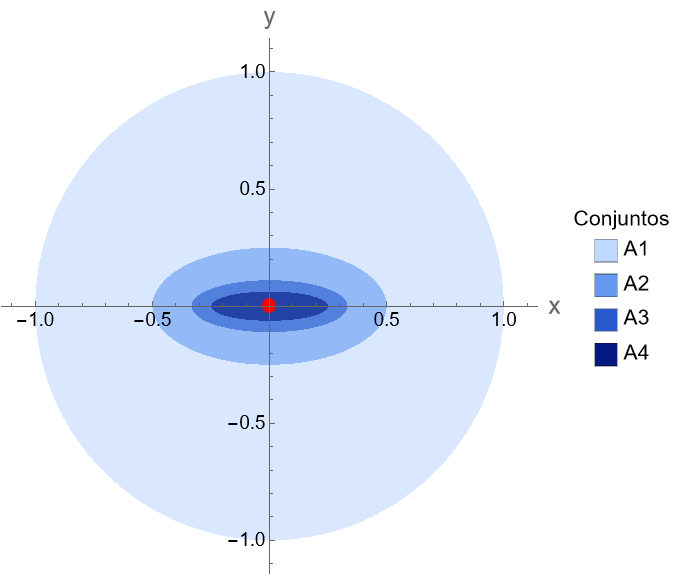
\includegraphics[width=0.55\linewidth]{imagenes/problemas_Quesada/prob_quesada_1_18_a}
\end{center}

    \item \textbf{Estudio de la sucesión de semiplanos $A_n$:}
    
    La sucesión oscila según la paridad del índice $n$:
    \begin{itemize}
        \item Para índices impares ($n = 2k-1$): $A_{2k-1} = \{ (x,y) \in \mathbb{R}^2 \mid x + y > -1 \} \equiv H_1$
        \item Para índices pares ($n = 2k$): $A_{2k} = \{ (x,y) \in \mathbb{R}^2 \mid x + y > 1 \} \equiv H_2$
    \end{itemize}
    
    Observamos la relación de inclusión estricta entre ambos semiplanos: $H_2 \subset H_1$ (ya que $x+y > 1 \implies x+y > -1$).
    
    Calculamos los límites superior e inferior descomponiendo en sus subsucesiones pares e impares:
    \begin{align*}
        \varlimsup_{n \to \infty} A_n &= \varlimsup_{n \to \infty} A_{2n-1} \cup \varlimsup_{n \to \infty} A_{2n} = H_1 \cup H_2 = H_1 = \{ (x,y) \in \mathbb{R}^2 \mid x + y > -1 \} \\
        \varliminf_{n \to \infty} A_n &= \varliminf_{n \to \infty} A_{2n-1} \cap \varliminf_{n \to \infty} A_{2n} = H_1 \cap H_2 = H_2 = \{ (x,y) \in \mathbb{R}^2 \mid x + y > 1 \}
    \end{align*}
    
    Al ser $\varlimsup_{n \to \infty} A_n \neq \varliminf_{n \to \infty} A_n$, la sucesión $\{A_n\}$ no es convergente.

    % --------------------------------------------------------------------------
    % HUECO RESERVADO PARA DIAGRAMA (APARTADO B)
    % --------------------------------------------------------------------------
    \begin{center}
        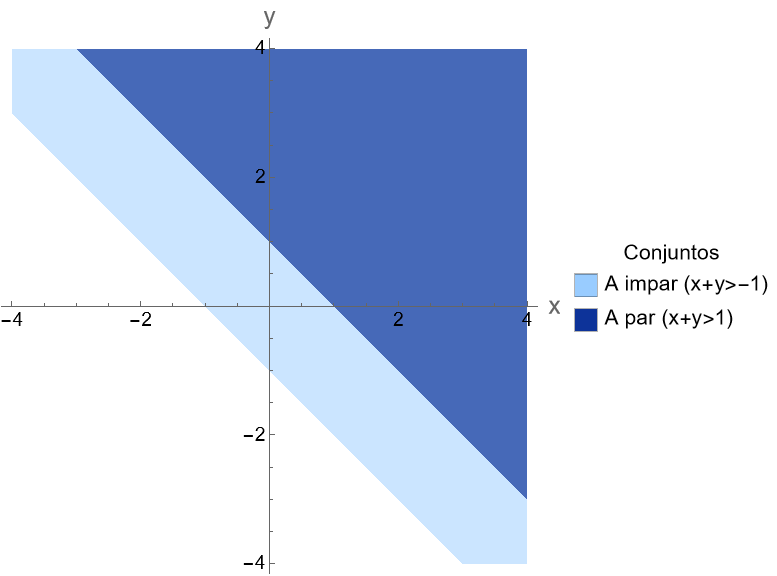
\includegraphics[width=0.55\linewidth]{imagenes/problemas_Quesada/prob_quesada_1_18_b}
    \end{center}
\end{enumerate}
\end{problema}
\newpage
% ------------------------------------------------------------------------------
% PROBLEMA 19
% ------------------------------------------------------------------------------
\begin{problema}[Límite de una sucesión de discos con centros oscilantes]
Sea la sucesión de círculos (discos cerrados) en $\mathbb{R}^2$:
\[
    C_n = \left\{ (x,y) \in \mathbb{R}^2 \,\,\middle|\,\, x^2 + \left(y - \left(-\frac{1}{2}\right)^n\right)^2 \le 1 \right\}
\]
Calcular su límite, si existe.

\tcblower

Sea $y_n = \left(-\frac{1}{2}\right)^n$. La sucesión $\{C_n\}_{n \in \mathbb{N}}$ consta de discos de radio $1$ centrados en $(0, y_n)$, donde la coordenada vertical del centro oscila en signo y tiende a $0$ cuando $n \to \infty$.

Para determinar si existe el límite, calculamos los límites inferior y superior de la sucesión analizando la condición de pertenencia de un punto $(x,y) \in \mathbb{R}^2$:
\[
    (x,y) \in C_n \iff x^2 + (y - y_n)^2 \le 1 \iff x^2 + y^2 - 2y y_n + y_n^2 \le 1
\]

Distinguimos tres regiones en el plano respecto al disco unidad centrado en el origen, $C = \{(x,y) \in \mathbb{R}^2 \mid x^2 + y^2 \le 1\}$:

\begin{enumerate}[label=\arabic*.]
    \item \textit{Puntos interiores ($x^2 + y^2 < 1$):}
    Existe $\varepsilon > 0$ tal que $x^2 + y^2 = 1 - \varepsilon$. Como $-2y y_n + y_n^2 \to 0$ cuando $n \to \infty$, existe $N \in \mathbb{N}$ tal que para todo $n \ge N$ se cumple $|-2y y_n + y_n^2| < \varepsilon$. 
    
    Por tanto, $x^2 + (y - y_n)^2 < 1$ para todo $n \ge N$, lo que implica que el punto pertenece a todos los conjuntos salvo a un número finito:
    \[
        \{(x,y) \in \mathbb{R}^2 \mid x^2 + y^2 < 1\} \subseteq \varliminf_{n \to \infty} C_n
    \]

    \item \textit{Puntos exteriores ($x^2 + y^2 > 1$):}
    Existe $\varepsilon > 0$ tal que $x^2 + y^2 = 1 + \varepsilon$. Análogamente, para $n$ suficientemente grande se cumple $x^2 + (y - y_n)^2 > 1$. Por consiguiente, el punto no pertenece a $C_n$ salvo para un número finito de índices, luego no forma parte del límite superior:
    \[
        \varlimsup_{n \to \infty} C_n \subseteq \{(x,y) \in \mathbb{R}^2 \mid x^2 + y^2 \le 1\}
    \]

    \item \textit{Puntos de la frontera ($x^2 + y^2 = 1$):}
    Sustituyendo $x^2 + y^2 = 1$, la condición $(x,y) \in C_n$ se reduce a $y_n(2y - y_n) \ge 0$.
    \begin{itemize}
        \item Si $y = 0$ (puntos $(1,0)$ y $(-1,0)$): La condición se convierte en $-y_n^2 \ge 0$, lo cual es falso para todo $n \in \mathbb{N}$. Por tanto, $(1,0)$ y $(-1,0)$ no pertenecen a ningún $C_n$.
        \item Si $y > 0$: Para $n$ par ($y_n > 0$), se cumple $2y - y_n > 0$ para $n$ grande, luego $y_n(2y - y_n) > 0$ y el punto pertenece a $C_n$. Para $n$ impar ($y_n < 0$), $y_n(2y - y_n) < 0$ y el punto no pertenece a $C_n$.
        \item Si $y < 0$: Análogamente, el punto pertenece a $C_n$ para $n$ impar suficientemente grande, pero no pertenece a $C_n$ para $n$ par.
    \end{itemize}
\end{enumerate}

En consecuencia, los límites inferior y superior vienen dados por:
\[
    \varliminf_{n \to \infty} C_n = \left\{ (x,y) \in \mathbb{R}^2 \,\,\middle|\,\, x^2 + y^2 < 1 \right\}
\]
\[
    \varlimsup_{n \to \infty} C_n = \left\{ (x,y) \in \mathbb{R}^2 \,\,\middle|\,\, x^2 + y^2 < 1 \right\} \cup \left\{ (x,y) \in \mathbb{R}^2 \,\,\middle|\,\, x^2 + y^2 = 1, \, y \neq 0 \right\}
\]

Puesto que $\varliminf_{n \to \infty} C_n \neq \varlimsup_{n \to \infty} C_n$, se concluye que la sucesión $\{C_n\}$ \textbf{no es convergente} y el límite $\displaystyle \lim_{n \to \infty} C_n$ \textbf{no existe}.

% --------------------------------------------------------------------------
% HUECO RESERVADO PARA DIAGRAMA
% --------------------------------------------------------------------------
\begin{center}
    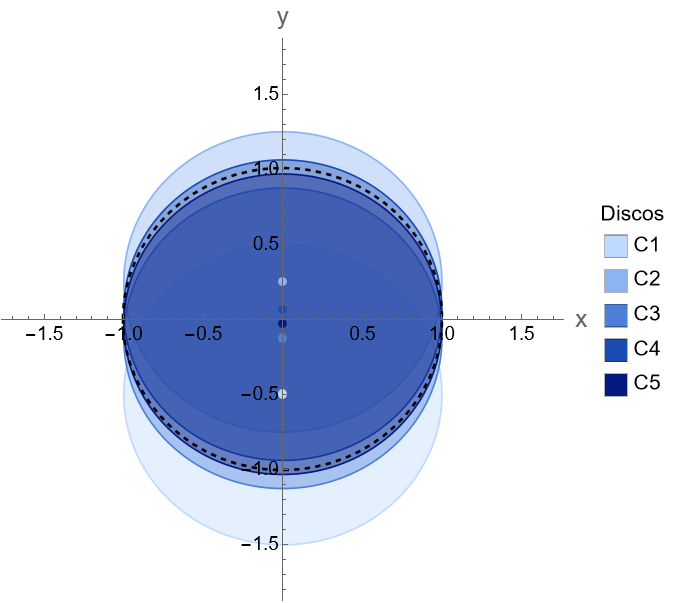
\includegraphics[width=0.55\linewidth]{imagenes/problemas_Quesada/prob_quesada_1_19_a}
\end{center}
\end{problema}
\newpage
% ------------------------------------------------------------------------------
% PROBLEMA 20
% ------------------------------------------------------------------------------
\begin{problema}[$\sigma$-álgebra de parejas de enteros contiguos]
Sea $\Omega = \mathbb{Z}^+$ y sea $\mathcal{A}$ la clase de subconjuntos de $\mathbb{Z}^+$ definida por:
\[
    \mathcal{A} = \{ A \subseteq \mathbb{Z}^+ \mid \forall n, \, 2n \in A \iff 2n+1 \in A \}
\]
Demostrar que $\mathcal{A}$ es una $\sigma$-álgebra sobre $\mathbb{Z}^+$.

\tcblower

\paragraph{Interpretación estructurada:}
La condición $2n \in A \iff 2n+1 \in A$ establece que los elementos de $\mathbb{Z}^+$ están agrupados en bloques o parejas indivisibles de la forma $P_n = \{2n, 2n+1\}$. Así, un subconjunto $A$ pertenece a $\mathcal{A}$ si y solo si es la unión de bloques completos $P_n$.

\begin{center}
    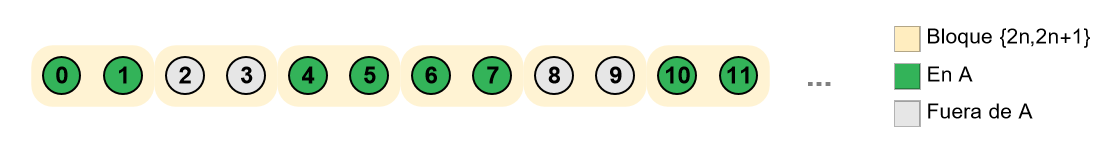
\includegraphics[width=0.75\linewidth]{imagenes/problemas_Quesada/prob_quesada_1_20_a}
\end{center}

Verificamos que la clase $\mathcal{A}$ satisface los tres axiomas de $\sigma$-álgebra:

\begin{enumerate}[label=\alph*)]
    \item \textbf{Pertenencia del conjunto universal:}
    Para todo $n$, los elementos $2n$ y $2n+1$ pertenecen trivialmente al espacio universal $\mathbb{Z}^+$. Por tanto, las proposiciones $2n \in \mathbb{Z}^+$ y $2n+1 \in \mathbb{Z}^+$ son ambas verdaderas, verificándose la equivalencia $2n \in \mathbb{Z}^+ \iff 2n+1 \in \mathbb{Z}^+$. Concluimos que:
    \[
        \mathbb{Z}^+ \in \mathcal{A}
    \]

    \item \textbf{Cierre por complementación:}
    Sea $A \in \mathcal{A}$. Para estudiar si su complementario $A^c = \mathbb{Z}^+ \setminus A$ pertenece a $\mathcal{A}$, evaluamos la condición para un entero $n$ cualquiera:
    \[
        2n \in A^c \iff 2n \notin A \iff \neg (2n \in A)
    \]
    Dado que $A \in \mathcal{A}$, se cumple $2n \in A \iff 2n+1 \in A$. Negando ambos miembros de la equivalencia:
    \[
        \neg (2n \in A) \iff \neg (2n+1 \in A) \iff 2n+1 \notin A \iff 2n+1 \in A^c
    \]
    Por tanto, $2n \in A^c \iff 2n+1 \in A^c$, lo que demuestra que:
    \[
        A^c \in \mathcal{A}
    \]

    \item \textbf{Cierre por uniones numerables:}
    Sea $\{A_k\}_{k \in \mathbb{N}} \subseteq \mathcal{A}$ una colección numerable de conjuntos. Definimos la unión numerable $A = \bigcup_{k=1}^\infty A_k$.
    
    Para cualquier entero $n$, se deducen las siguientes equivalencias lógicas:
    \begin{align*}
        2n \in \bigcup_{k=1}^\infty A_k &\iff \exists k_0 \in \mathbb{N} \text{ tal que } 2n \in A_{k_0} \\
        &\iff \exists k_0 \in \mathbb{N} \text{ tal que } 2n+1 \in A_{k_0} \quad (\text{pues } A_{k_0} \in \mathcal{A}) \\
        &\iff 2n+1 \in \bigcup_{k=1}^\infty A_k
    \end{align*}
    Al cumplirse la equivalencia $2n \in A \iff 2n+1 \in A$, concluimos que:
    \[
        \bigcup_{k=1}^\infty A_k \in \mathcal{A}
    \]
\end{enumerate}

Al verificarse las tres condiciones, queda demostrado que la clase $\mathcal{A}$ es una $\sigma$-álgebra sobre $\mathbb{Z}^+$.

\end{problema}
\newpage
% ------------------------------------------------------------------------------
% PROBLEMA 21
% ------------------------------------------------------------------------------
\begin{problema}[$\sigma$-álgebra co-numerable]
Sea $\Omega$ un conjunto no numerable y sea la clase de subconjuntos
\[
    \mathcal{C} = \{ A \in \mathcal{P}(\Omega) \mid A \text{ o } A^c \text{ es numerable} \}
\]
Demostrar que $\mathcal{C}$ es una $\sigma$-álgebra sobre $\Omega$.

\tcblower

Verificamos que la clase $\mathcal{C}$ cumple las tres condiciones características de una $\sigma$-álgebra sobre $\Omega$:

\begin{enumerate}[label=\alph*)]
    \item \textbf{Pertenencia del conjunto universal:}
    El complementario del espacio universal $\Omega$ es el conjunto vacío, $\Omega^c = \varnothing$. Puesto que el conjunto vacío es finito (y, por tanto, numerable), se deduce directamente que:
    \[
        \Omega \in \mathcal{C}
    \]

    \item \textbf{Cierre por complementación:}
    Sea $A \in \mathcal{C}$. Por definición de la clase $\mathcal{C}$, se verifica que $A$ es numerable o $A^c$ es numerable.
    
    Analizamos el complementario $A^c$, teniendo en cuenta la propiedad de la doble complementación $(A^c)^c = A$:
    \begin{itemize}
        \item Si $A$ es numerable, entonces $(A^c)^c$ es numerable, luego $A^c \in \mathcal{C}$.
        \item Si $A^c$ es numerable, por definición directa se tiene $A^c \in \mathcal{C}$.
    \end{itemize}
    En cualquiera de los dos casos, $A^c \in \mathcal{C}$.

    \item \textbf{Cierre por uniones numerables:}
    Sea $\{A_n\}_{n \in \mathbb{N}} \subseteq \mathcal{C}$ una colección numerable de conjuntos. Distinguimos dos casos posibles:
    \begin{itemize}
        \item \textit{Caso 1: Todos los conjuntos $A_n$ son numerables.}
        Puesto que la unión numerable de conjuntos numerables es a su vez numerable, la unión $\bigcup_{n=1}^\infty A_n$ es numerable, por lo que:
        \[
            \bigcup_{n=1}^\infty A_n \in \mathcal{C}
        \]

        \item \textit{Caso 2: Existe al menos un índice $n_0 \in \mathbb{N}$ tal que $A_{n_0}$ no es numerable.}
        Al ser $A_{n_0} \in \mathcal{C}$, necesariamente su complementario $A_{n_0}^c$ debe ser numerable. Aplicando las leyes de De Morgan:
        \[
            \left( \bigcup_{n=1}^\infty A_n \right)^c = \bigcap_{n=1}^\infty A_n^c \subseteq A_{n_0}^c
        \]
        Puesto que cualquier subconjunto de un conjunto numerable es numerable, el complementario $\left( \bigcup_{n=1}^\infty A_n \right)^c$ es numerable, concluyendo que:
        \[
            \bigcup_{n=1}^\infty A_n \in \mathcal{C}
        \]
    \end{itemize}
\end{enumerate}

Al satisfacerse las tres propiedades, queda demostrado que $\mathcal{C}$ es una $\sigma$-álgebra sobre $\Omega$.

\end{problema}
\newpage
% ------------------------------------------------------------------------------
% PROBLEMA 22
% ------------------------------------------------------------------------------
\begin{problema}[$\sigma$-álgebra generada por una partición numerable]
Dado un conjunto universal $\Omega$, sea $\mathcal{A} = \{A_n\}_{n \in \mathbb{N}}$ una familia numerable de subconjuntos de $\Omega$, disjuntos dos a dos y tales que $\bigcup_{n \in \mathbb{N}} A_n = \Omega$. Demostrar que la $\sigma$-álgebra generada por $\mathcal{A}$, denotada por $\sigma(\mathcal{A})$, coincide con la clase $\mathcal{C}$ formada por todas las uniones arbitrarias de elementos de la familia:
\[
    \mathcal{C} = \left\{ \bigcup_{n \in I} A_n \,\,\middle|\,\, I \subseteq \mathbb{N} \right\}
\]

\tcblower

Para demostrar la igualdad $\sigma(\mathcal{A}) = \mathcal{C}$, establecemos la doble inclusión entre ambas clases:

\begin{enumerate}[label=\arabic*.]
    \item \textbf{Inclusión $\sigma(\mathcal{A}) \subseteq \mathcal{C}$:}
    
    Basta verificar que $\mathcal{C}$ es una $\sigma$-álgebra sobre $\Omega$ que contiene a la familia de generadores $\mathcal{A}$:
    \begin{enumerate}[label=\alph*)]
        \item \textit{Pertenencia de $\Omega$:} Tomando el subconjunto de índices $I = \mathbb{N}$, se tiene $\Omega = \bigcup_{n \in \mathbb{N}} A_n \in \mathcal{C}$.
        
        \item \textit{Cierre por complementación:} Sea $C = \bigcup_{n \in I} A_n \in \mathcal{C}$. Dado que la familia $\{A_n\}_{n \in \mathbb{N}}$ constituye una partición disjunta de $\Omega$, el complementario de $C$ es la unión de los bloques restantes:
        \[
            C^c = \Omega \setminus \left( \bigcup_{n \in I} A_n \right) = \bigcup_{n \in \mathbb{N} \setminus I} A_n
        \]
        Como $\mathbb{N} \setminus I \subseteq \mathbb{N}$, se sigue inmediatamente que $C^c \in \mathcal{C}$.
        \begin{center}
            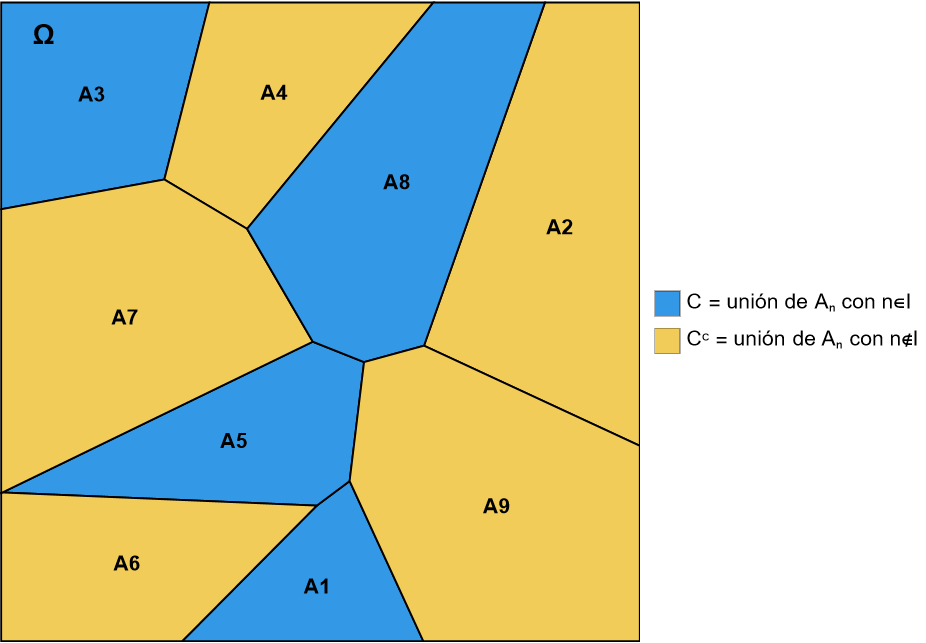
\includegraphics[width=0.55\linewidth]{imagenes/problemas_Quesada/prob_quesada_1_22_a}
        \end{center}

        \item \textit{Cierre por uniones numerables:} Sea $\{C_k\}_{k \in \mathbb{N}} \subseteq \mathcal{C}$, donde cada $C_k = \bigcup_{n \in I_k} A_n$ para algún subconjunto de índices $I_k \subseteq \mathbb{N}$. La unión numerable resulta:
        \[
            \bigcup_{k=1}^\infty C_k = \bigcup_{k=1}^\infty \left( \bigcup_{n \in I_k} A_n \right) = \bigcup_{n \in \bigcup_{k=1}^\infty I_k} A_n
        \]
        Al ser $\bigcup_{k=1}^\infty I_k \subseteq \mathbb{N}$, la unión pertenece a $\mathcal{C}$.
    \end{enumerate}
    
    Así, $\mathcal{C}$ es una $\sigma$-álgebra. Además, tomando $I = \{n\}$ para cada $n \in \mathbb{N}$, tenemos que $A_n \in \mathcal{C}$, de modo que $\mathcal{A} \subseteq \mathcal{C}$. Como $\sigma(\mathcal{A})$ es la minimal entre las $\sigma$-álgebras que contienen a $\mathcal{A}$, concluimos que:
    \[
        \sigma(\mathcal{A}) \subseteq \mathcal{C}
    \]

    \item \textbf{Inclusión $\mathcal{C} \subseteq \sigma(\mathcal{A})$:}
    
    Sea $C = \bigcup_{n \in I} A_n \in \mathcal{C}$ un elemento cualquiera de la clase. Por definición, cada bloque $A_n$ pertenece a la familia generadora $\mathcal{A} \subseteq \sigma(\mathcal{A})$.
    
    Puesto que $I \subseteq \mathbb{N}$ es un conjunto a lo sumo numerable de índices y la $\sigma$-álgebra $\sigma(\mathcal{A})$ es cerrada por uniones numerables, la unión $\bigcup_{n \in I} A_n$ pertenece necesariamente a $\sigma(\mathcal{A})$. Por tanto:
    \[
        \mathcal{C} \subseteq \sigma(\mathcal{A})
    \]
\end{enumerate}

De la combinación de ambas inclusiones se deduce que $\sigma(\mathcal{A}) = \mathcal{C}$.
\end{problema}

\newpage
%=====================================================
%=========== TEMA 2. ESPACIO PROBABILÍSTICO ==========
%=====================================================
\section{Espacio probabilístico}
\setcounter{problemacontador}{0}
% ------------------------------------------------------------------------------
% PROBLEMA 1
% ------------------------------------------------------------------------------
\begin{problema}[Mezcla de una colección numerable de medidas de probabilidad]
Sea $(\Omega, \mathcal{Q})$ un espacio probabilizable y sea $(P_n)_{n \in \mathbb{N}}$ una sucesión de medidas de probabilidad definidas sobre él. Demostrar que la función de conjunto
\[
    P(A) = \sum_{n=1}^\infty a_n P_n(A)
\]
es una medida de probabilidad sobre el mismo espacio, para cualquier sucesión de números reales $(a_n)_{n \in \mathbb{N}}$ tal que $a_n \ge 0$ para todo $n \in \mathbb{N}$ y $\displaystyle \sum_{n=1}^\infty a_n = 1$.

\tcblower

Comprobamos que la función de conjunto $P : \mathcal{Q} \to \mathbb{R}$ satisface los tres axiomas de Kolmogorov para ser una medida de probabilidad:\\[4pt]
\noindent
\textbf{1. No negatividad:}
Para cualquier suceso $A \in \mathcal{Q}$, dado que $a_n \ge 0$ y $P_n(A) \ge 0$ para todo $n \in \mathbb{N}$ (por ser cada $P_n$ una medida de probabilidad), cada término del sumatorio cumple $a_n P_n(A) \ge 0$.
La suma de términos no negativos es no negativa, por lo que:
\[
    P(A) = \sum_{n=1}^\infty a_n P_n(A) \ge 0, \quad \forall A \in \mathcal{Q}
\]
\noindent
\textbf{2. Normalización del espacio muestral:}\\
Evaluamos la función $P$ sobre el conjunto universal $\Omega$. Dado que $P_n(\Omega) = 1$ para todo $n \in \mathbb{N}$ y $\displaystyle \sum_{n=1}^\infty a_n = 1$:
\[
    P(\Omega) = \sum_{n=1}^\infty a_n P_n(\Omega) = \sum_{n=1}^\infty a_n \cdot 1 = \sum_{n=1}^\infty a_n = 1
\]

\begin{center}
    \includegraphics[width=1\linewidth]{imagenes/problemas_Quesada/prob_quesada_2_1_a}
\end{center}
\noindent
\textbf{3. $\sigma$-aditividad:}\\
Sea $(A_i)_{i \in \mathbb{N}} \subseteq \mathcal{Q}$ una sucesión de sucesos disjuntos dos a dos ($A_i \cap A_j = \varnothing$ para todo $i \neq j$).
Por la $\sigma$-aditividad de cada medida $P_n$, se tiene que $P_n\left(\bigcup_{i=1}^\infty A_i\right) = \sum_{i=1}^\infty P_n(A_i)$.
Sustituyendo esta propiedad en la definición de la función $P$:
\[
    P\left( \bigcup_{i=1}^\infty A_i \right) = \sum_{n=1}^\infty a_n P_n\left( \bigcup_{i=1}^\infty A_i \right) = \sum_{n=1}^\infty a_n \left( \sum_{i=1}^\infty P_n(A_i) \right) = \sum_{n=1}^\infty \sum_{i=1}^\infty a_n P_n(A_i)
\]
Puesto que todos los términos $a_n P_n(A_i)$ son no negativos, podemos aplicar el Teorema de Tonelli para series dobles (intercambio del orden de sumación para términos no negativos) sin alterar la convergencia ni la suma:
\[
    \sum_{n=1}^\infty \sum_{i=1}^\infty a_n P_n(A_i) = \sum_{i=1}^\infty \sum_{n=1}^\infty a_n P_n(A_i) = \sum_{i=1}^\infty P(A_i)
\]
Concluimos que:
\[
    P\left( \bigcup_{i=1}^\infty A_i \right) = \sum_{i=1}^\infty P(A_i)
\]

Al cumplirse los tres axiomas, queda demostrado que $P$ es una medida de probabilidad sobre $(\Omega, \mathcal{Q})$.
\end{problema}

\newpage

% ------------------------------------------------------------------------------
% PROBLEMA 2
% ------------------------------------------------------------------------------
\begin{problema}[Propiedades de la probabilidad y diferencia simétrica]
Sea $(\Omega, \mathcal{Q}, P)$ un espacio de probabilidad y sean $A, B \in \mathcal{Q}$. Demostrar que:
\begin{enumerate}[label=\alph*)]
    \item $P(A) = P(B) = 1 \implies P(A \cap B) = P(A \cup B) = 1$
    \item $P(A \Delta B) = P(A) + P(B) - 2P(A \cap B)$
    \item $P(A \Delta B) = 0 \implies P(A) = P(B)$
\end{enumerate}

\tcblower

\paragraph{a)}
Por la propiedad de monotonía de la medida de probabilidad, al ser $A \subseteq A \cup B \subseteq \Omega$, se satisface la cadena de desigualdades:
\[
    1 = P(A) \le P(A \cup B) \le P(\Omega) = 1 \implies P(A \cup B) = 1
\]
Por otra parte, aplicando la fórmula de la probabilidad de la unión de dos sucesos:
\[
    P(A \cup B) = P(A) + P(B) - P(A \cap B) \implies 1 = 1 + 1 - P(A \cap B) \implies P(A \cap B) = 1
\]
Por tanto, se concluye que $P(A \cap B) = P(A \cup B) = 1$.

\paragraph{b)}
La diferencia simétrica entre dos conjuntos se define equivalentemente como la diferencia entre su unión y su intersección:
\[
    A \Delta B = (A \cup B) \setminus (A \cap B)
\]
Dado que $(A \cap B) \subseteq (A \cup B)$, aplicando la propiedad de la probabilidad de la diferencia de conjuntos contenidos:
\[
    P(A \Delta B) = P\bigl((A \cup B) \setminus (A \cap B)\bigr) = P(A \cup B) - P(A \cap B)
\]
Sustituyendo la fórmula general para la unión $P(A \cup B) = P(A) + P(B) - P(A \cap B)$:
\[
    P(A \Delta B) = P(A) + P(B) - P(A \cap B) - P(A \cap B) = P(A) + P(B) - 2P(A \cap B)
\]

\begin{center}
    \includegraphics[width=0.5\linewidth]{imagenes/problemas_Quesada/prob_quesada_2_2_a}
\end{center}

\paragraph{c)}
Supongamos que $P(A \Delta B) = 0$. Utilizando la igualdad demostrada en el apartado anterior:
\[
    P(A \cup B) - P(A \cap B) = 0 \implies P(A \cap B) = P(A \cup B)
\]
Por las inclusiones de conjuntos $A \cap B \subseteq A \subseteq A \cup B$ y $A \cap B \subseteq B \subseteq A \cup B$, la monotonía de la probabilidad establece que:
\[
    P(A \cap B) \le P(A) \le P(A \cup B) \quad \text{y} \quad P(A \cap B) \le P(B) \le P(A \cup B)
\]
Al coincidir el valor de los extremos inferior y superior ($P(A \cap B) = P(A \cup B)$), las desigualdades se saturan como igualdades, deduciéndose directamente que:
\[
    P(A) = P(A \cap B) = P(B) = P(A \cup B)
\]
Por consiguiente, $P(A) = P(B)$.
\end{problema}

\newpage

% ------------------------------------------------------------------------------
% PROBLEMA 3
% ------------------------------------------------------------------------------
\begin{problema}[Verificación del axioma de normalización mediante integración]
Se define la función de conjunto $P$ sobre el espacio medible $(\mathbb{R}, \mathcal{B}(\mathbb{R}))$ del siguiente modo:
\[
    P(B) = \int_{B \cap [1, \infty)} \frac{1}{2} \, dx, \quad \forall B \in \mathcal{B}(\mathbb{R})
\]
¿Es $P$ una probabilidad sobre $(\mathbb{R}, \mathcal{B}(\mathbb{R}))$?

\tcblower

\paragraph{Respuesta:}
No, $P$ no es una medida de probabilidad sobre $(\mathbb{R}, \mathcal{B}(\mathbb{R}))$.\\[4pt]
Para determinar si $P$ es una medida de probabilidad, analizamos el cumplimiento de los tres axiomas de Kolmogorov:

\paragraph{1. No negatividad:}
Como el integrando $f(x) = \frac{1}{2}$ es estrictamente positivo y la medida de Lebesgue es positiva, la integral sobre cualquier región medible $B \cap [1, \infty)$ resulta no negativa:
\[
    P(B) = \int_{B \cap [1, \infty)} \frac{1}{2} \, dx \ge 0, \quad \forall B \in \mathcal{B}(\mathbb{R})
\]

\paragraph{2. $\sigma$-aditividad:}
Dada una colección numerable de sucesos borelianos disjuntos dos a dos $(B_n)_{n \in \mathbb{N}} \subseteq \mathcal{B}(\mathbb{R})$ ($B_i \cap B_j = \varnothing$ para $i \neq j$), la intersección con $[1, \infty)$ preserva el disjuntismo. Por la $\sigma$-aditividad de la integral de Lebesgue (o el Teorema de Convergencia Monótona):
\[
    \begin{array}{rl}
        \displaystyle P\left( \bigcup_{n=1}^\infty B_n \right) & \displaystyle = \int_{\left(\bigcup_{n=1}^\infty B_n\right) \cap [1, \infty)} \frac{1}{2} \, dx = \int_{\bigcup_{n=1}^\infty \left(B_n \cap [1, \infty)\right)} \frac{1}{2} \, dx \\[16pt]
        & \displaystyle = \sum_{n=1}^\infty \int_{B_n \cap [1, \infty)} \frac{1}{2} \, dx = \sum_{n=1}^\infty P(B_n)
    \end{array}
\]

\paragraph{3. Normalización del espacio muestral:}
Evaluamos la medida sobre todo el conjunto universal $\Omega = \mathbb{R}$:
\[
    P(\mathbb{R}) = \int_{\mathbb{R} \cap [1, \infty)} \frac{1}{2} \, dx = \int_{1}^{\infty} \frac{1}{2} \, dx = \left[ \frac{x}{2} \right]_{1}^{\infty} = \infty
\]
Puesto que $P(\mathbb{R}) = \infty \neq 1$, no se satisface la condición de estar normada a la unidad.
\vspace{1cm}
\begin{center}
    
\includegraphics[width=1\linewidth]{imagenes/problemas_Quesada/prob_quesada_2_3_a}
\end{center}
 
\paragraph{Conclusión:}
Aunque $P$ define una medida sobre el espacio medible $(\mathbb{R}, \mathcal{B}(\mathbb{R}))$, al no cumplir el axioma de normalización ($P(\mathbb{R}) \neq 1$), no constituye una medida de probabilidad.
\end{problema}

\newpage

% ------------------------------------------------------------------------------
% PROBLEMA 4
% ------------------------------------------------------------------------------
\begin{problema}[Medida de probabilidad inducida por una densidad]
Sea $\Omega = [0,1]$. Supongamos que sobre la $\sigma$-álgebra de Borel $\mathcal{B}([0,1])$ definimos una aplicación $P$ dada por:
\[
    P(B) = \int_B f(x) \, dx, \quad \forall B \in \mathcal{B}([0,1])
\]
donde $f : [0,1] \to \mathbb{R}$ es una función no negativa tal que $\displaystyle \int_0^1 f(x) \, dx = 1$.
\begin{enumerate}[label=\alph*)]
    \item Demostrar que $P$ es una medida de probabilidad sobre $([0,1], \mathcal{B}([0,1]))$.
    \item Demostrar que $P(\{r\}) = 0$ para todo $r \in [0,1]$.
    \item Calcular $P(\mathbb{Q} \cap [0,1])$, donde $\mathbb{Q}$ representa al conjunto de los números racionales.
    \item Demostrar que $P((a,b]) = P([a,b])$ para cualquier intervalo $[a,b] \subseteq [0,1]$.
\end{enumerate}

\tcblower

\paragraph{a)}
Comprobamos los tres axiomas de Kolmogorov para verificar que $P$ es una medida de probabilidad sobre el espacio medible $([0,1], \mathcal{B}([0,1]))$:
\begin{enumerate}[label=\arabic*.]
    \item \textbf{No negatividad:} Como $f(x) \ge 0$ para todo $x \in [0,1]$, la integral de una función no negativa sobre cualquier conjunto boreliano $B \in \mathcal{B}([0,1])$ resulta siempre no negativa:
    \[
        P(B) = \int_B f(x) \, dx \ge 0, \quad \forall B \in \mathcal{B}([0,1])
    \]
    \item \textbf{Normalización del espacio muestral:} Evaluamos la medida sobre el conjunto universal $\Omega = [0,1]$ aplicando la hipótesis dada:
    \[
        P([0,1]) = \int_0^1 f(x) \, dx = 1
    \]
    \item \textbf{$\sigma$-aditividad:} Dada una sucesión de conjuntos borelianos disjuntos dos a dos $(B_n)_{n \in \mathbb{N}} \subseteq \mathcal{B}([0,1])$ ($B_i \cap B_j = \varnothing$ para $i \neq j$), por la $\sigma$-aditividad de la integral de Lebesgue respecto del dominio de integración:
    \[
        P\left( \bigcup_{n=1}^\infty B_n \right) = \int_{\bigcup_{n=1}^\infty B_n} f(x) \, dx = \sum_{n=1}^\infty \int_{B_n} f(x) \, dx = \sum_{n=1}^\infty P(B_n)
    \]
\end{enumerate}
Por tanto, $P$ es una medida de probabilidad bien definida.

\paragraph{b)}
Dado un punto arbitrario $r \in [0,1]$, el conjunto unipuntual $\{r\}$ pertenece a $\mathcal{B}([0,1])$. Dado que la medida de Lebesgue de cualquier punto aislado es nula ($\lambda(\{r\}) = 0$), la integral de la función $f$ sobre dicho conjunto es cero:
\[
    P(\{r\}) = \int_{\{r\}} f(x) \, dx = 0
\]

\paragraph{c)}
El conjunto de los números racionales $\mathbb{Q}$ es numerable, de modo que la intersección $\mathbb{Q} \cap [0,1]$ es también un conjunto numerable. Por consiguiente, podemos expresar este conjunto como la unión numerable disjunta de sus puntos individuales:
\[
    \mathbb{Q} \cap [0,1] = \bigcup_{r \in \mathbb{Q} \cap [0,1]} \{r\}
\]
Aplicando la propiedad de $\sigma$-aditividad demostrada en el apartado a) junto con el resultado del apartado b):
\[
    P(\mathbb{Q} \cap [0,1]) = \sum_{r \in \mathbb{Q} \cap [0,1]} P(\{r\}) = \sum_{r \in \mathbb{Q} \cap [0,1]} 0 = 0
\]

\paragraph{d)}
Dado un intervalo $[a,b] \subseteq [0,1]$, podemos expresar el intervalo cerrado como la unión disjunta de su extremo izquierdo y del intervalo semiabierto correspondiente:
\[
    [a,b] = \{a\} \cup (a,b] \quad \text{con } \{a\} \cap (a,b] = \varnothing
\]
Por la aditividad de la probabilidad $P$:
\[
    P([a,b]) = P(\{a\}) + P((a,b])
\]
Puesto que $P(\{a\}) = 0$ por el apartado b), concluimos directamente que:
\[
    P([a,b]) = 0 + P((a,b]) = P((a,b])
\]
\vspace{1cm}
\begin{center}
    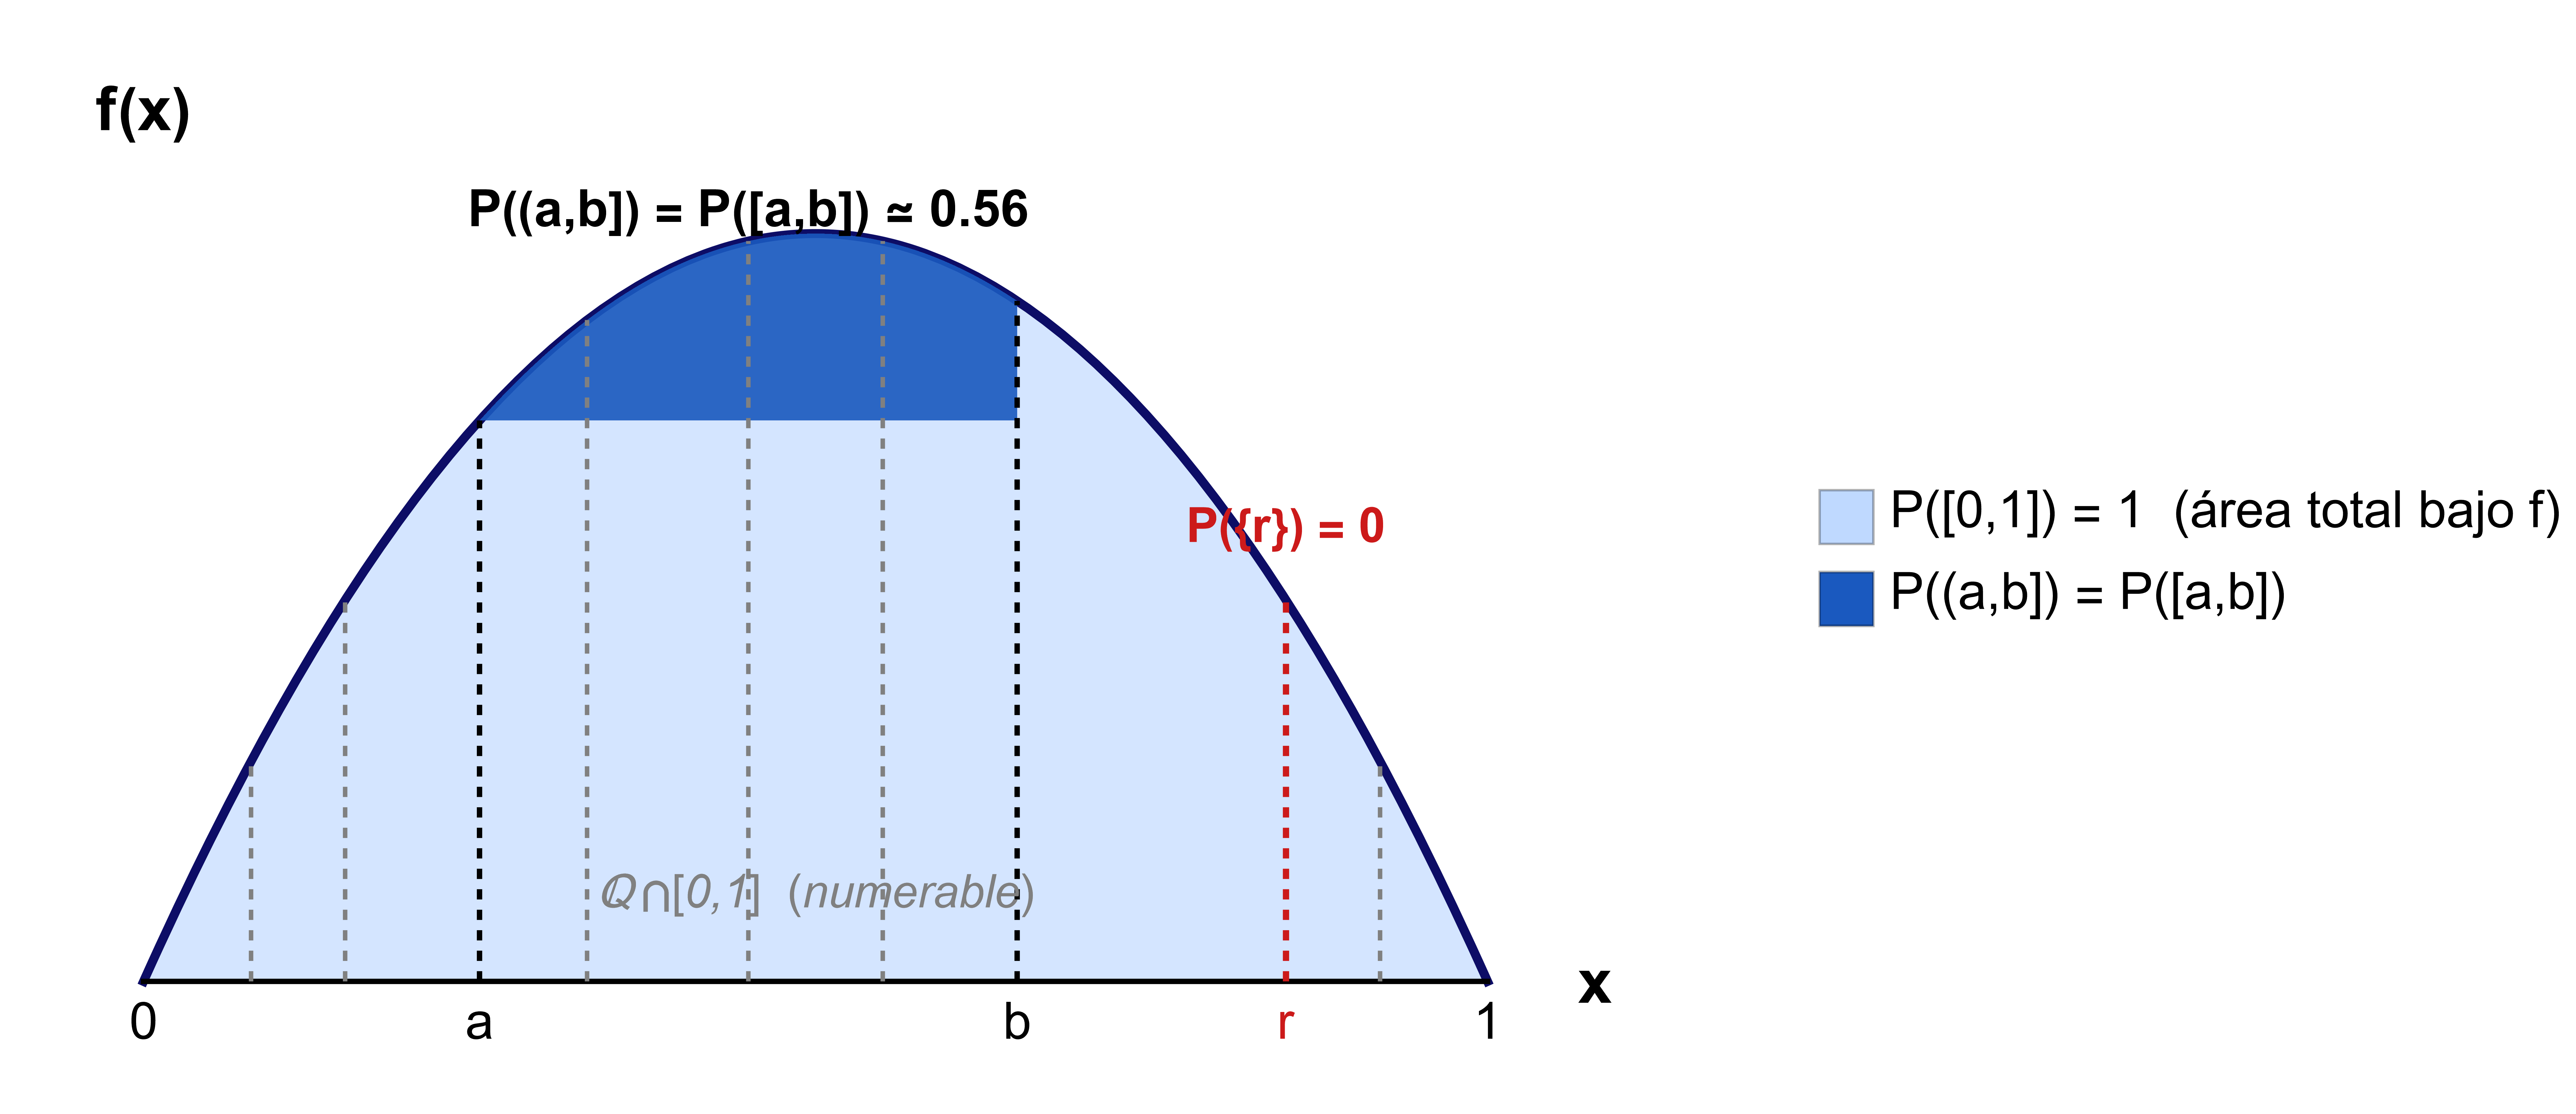
\includegraphics[width=1\linewidth]{imagenes/problemas_Quesada/prob_quesada_2_4_a}
\end{center}
\end{problema}

\newpage

% ------------------------------------------------------------------------------
% PROBLEMA 5
% ------------------------------------------------------------------------------
\begin{problema}[Espacio de probabilidad para el lanzamiento de dos dados]
Se lanzan al azar dos dados ($a$ y $b$), y denotamos por $\Omega_a = \{1,2,3,4,5,6\}$ y $\Omega_b = \{1,2,3,4,5,6\}$ los resultados elementales posibles en cada uno de ellos.
\begin{enumerate}[label=\alph*)]
    \item Comprobar que $(\Omega_a \times \Omega_b, \mathcal{P}(\Omega_a \times \Omega_b), P)$, donde $P(A \times B) = \frac{\text{card}(A) \cdot \text{card}(B)}{36}$ para todo $A \times B \in \mathcal{P}(\Omega_a) \times \mathcal{P}(\Omega_b)$, determina un espacio de probabilidad de sucesos elementales equiprobables.
    \item Demostrar que la aplicación $P_a : \mathcal{P}(\Omega_a) \to \mathbb{R}$ tal que $P_a(A) = P(A \times \Omega_b)$ es una medida de probabilidad sobre $(\Omega_a, \mathcal{P}(\Omega_a))$ y que sus sucesos elementales son equiprobables.
\end{enumerate}

\tcblower

\paragraph{a)}
El espacio muestral del experimento conjunto es el producto cartesiano $\Omega = \Omega_a \times \Omega_b$, cuyo cardinal es $\text{card}(\Omega) = 6 \cdot 6 = 36$. Dado que $\Omega$ es finito, la clase de las partes $\mathcal{P}(\Omega_a \times \Omega_b)$ constituye trivialmente una $\sigma$-álgebra sobre $\Omega$.

Consideremos los sucesos elementales unipuntuales $\{(i,j)\} = \{i\} \times \{j\}$ para $(i,j) \in \Omega_a \times \Omega_b$. Aplicando la definición dada sobre el producto de singletons:
\[
    P(\{(i,j)\}) = P(\{i\} \times \{j\}) = \frac{\text{card}(\{i\}) \cdot \text{card}(\{j\})}{36} = \frac{1 \cdot 1}{36} = \frac{1}{36}
\]
Dado que $P(\{(i,j)\}) = \frac{1}{36} > 0$ para todo $(i,j) \in \Omega$ y la suma de las probabilidades sobre todo el espacio es:
\[
    \sum_{(i,j) \in \Omega} P(\{(i,j)\}) = \sum_{i=1}^6 \sum_{j=1}^6 \frac{1}{36} = 36 \cdot \frac{1}{36} = 1
\]
queda inducida de manera única una medida de probabilidad sobre $(\Omega, \mathcal{P}(\Omega))$ dada por la regla de Laplace:
\[
    P(C) = \sum_{(i,j) \in C} P(\{(i,j)\}) = \frac{\text{card}(C)}{36}, \quad \forall C \subseteq \Omega
\]
Para un rectángulo medible $A \times B$, al cumplirse $\text{card}(A \times B) = \text{card}(A) \cdot \text{card}(B)$, la expresión coincide exactamente con la dada:
\[
    P(A \times B) = \frac{\text{card}(A) \cdot \text{card}(B)}{36}
\]
Por tanto, $(\Omega_a \times \Omega_b, \mathcal{P}(\Omega_a \times \Omega_b), P)$ determina un espacio de probabilidad discreto con sucesos elementales equiprobables.

\paragraph{b)}
Verificamos que $P_a : \mathcal{P}(\Omega_a) \to \mathbb{R}$ satisface los axiomas de Kolmogorov sobre el espacio muestral $(\Omega_a, \mathcal{P}(\Omega_a))$:
\begin{enumerate}[label=\arabic*.]
    \item \textbf{No negatividad:} Para cualquier $A \in \mathcal{P}(\Omega_a)$, por ser $P$ una medida de probabilidad:
    \[
        P_a(A) = P(A \times \Omega_b) \ge 0
    \]
    \item \textbf{Normalización:} Evaluamos sobre la totalidad del espacio fuente $\Omega_a$:
    \[
        P_a(\Omega_a) = P(\Omega_a \times \Omega_b) = \frac{\text{card}(\Omega_a) \cdot \text{card}(\Omega_b)}{36} = \frac{6 \cdot 6}{36} = 1
    \]
    \item \textbf{$\sigma$-aditividad:} Sea $(A_n)_{n \in \mathbb{N}} \subseteq \mathcal{P}(\Omega_a)$ una sucesión de sucesos disjuntos dos a dos ($A_i \cap A_j = \varnothing$ para $i \neq j$). Se tiene que los cilindros $(A_n \times \Omega_b)_{n \in \mathbb{N}}$ son disjuntos dos a dos en $\mathcal{P}(\Omega_a \times \Omega_b)$. Por la aditividad de $P$:
    \[
    \begin{array}{rl}
        P_a\left( \bigcup_{n=1}^\infty A_n \right) & \displaystyle = P\left( \left(\bigcup_{n=1}^\infty A_n\right) \times \Omega_b \right) = P\left( \bigcup_{n=1}^\infty (A_n \times \Omega_b) \right) = \\[12pt]
        & \displaystyle = \sum_{n=1}^\infty P(A_n \times \Omega_b) = \sum_{n=1}^\infty P_a(A_n)
    \end{array}
    \]
\end{enumerate}
Así pues, $P_a$ es una medida de probabilidad sobre $(\Omega_a, \mathcal{P}(\Omega_a))$.

Finalmente, evaluamos la probabilidad marginal $P_a$ sobre un suceso elemental arbitrario $\{i\} \subseteq \Omega_a$:
\[
    P_a(\{i\}) = P(\{i\} \times \Omega_b) = \frac{\text{card}(\{i\}) \cdot \text{card}(\Omega_b)}{36} = \frac{1 \cdot 6}{36} = \frac{1}{6}
\]
Puesto que $P_a(\{i\}) = \frac{1}{6}$ para todo $i \in \{1,2,3,4,5,6\}$, los sucesos elementales de $(\Omega_a, \mathcal{P}(\Omega_a))$ son equiprobables.
\vspace{1cm}
\begin{center}
    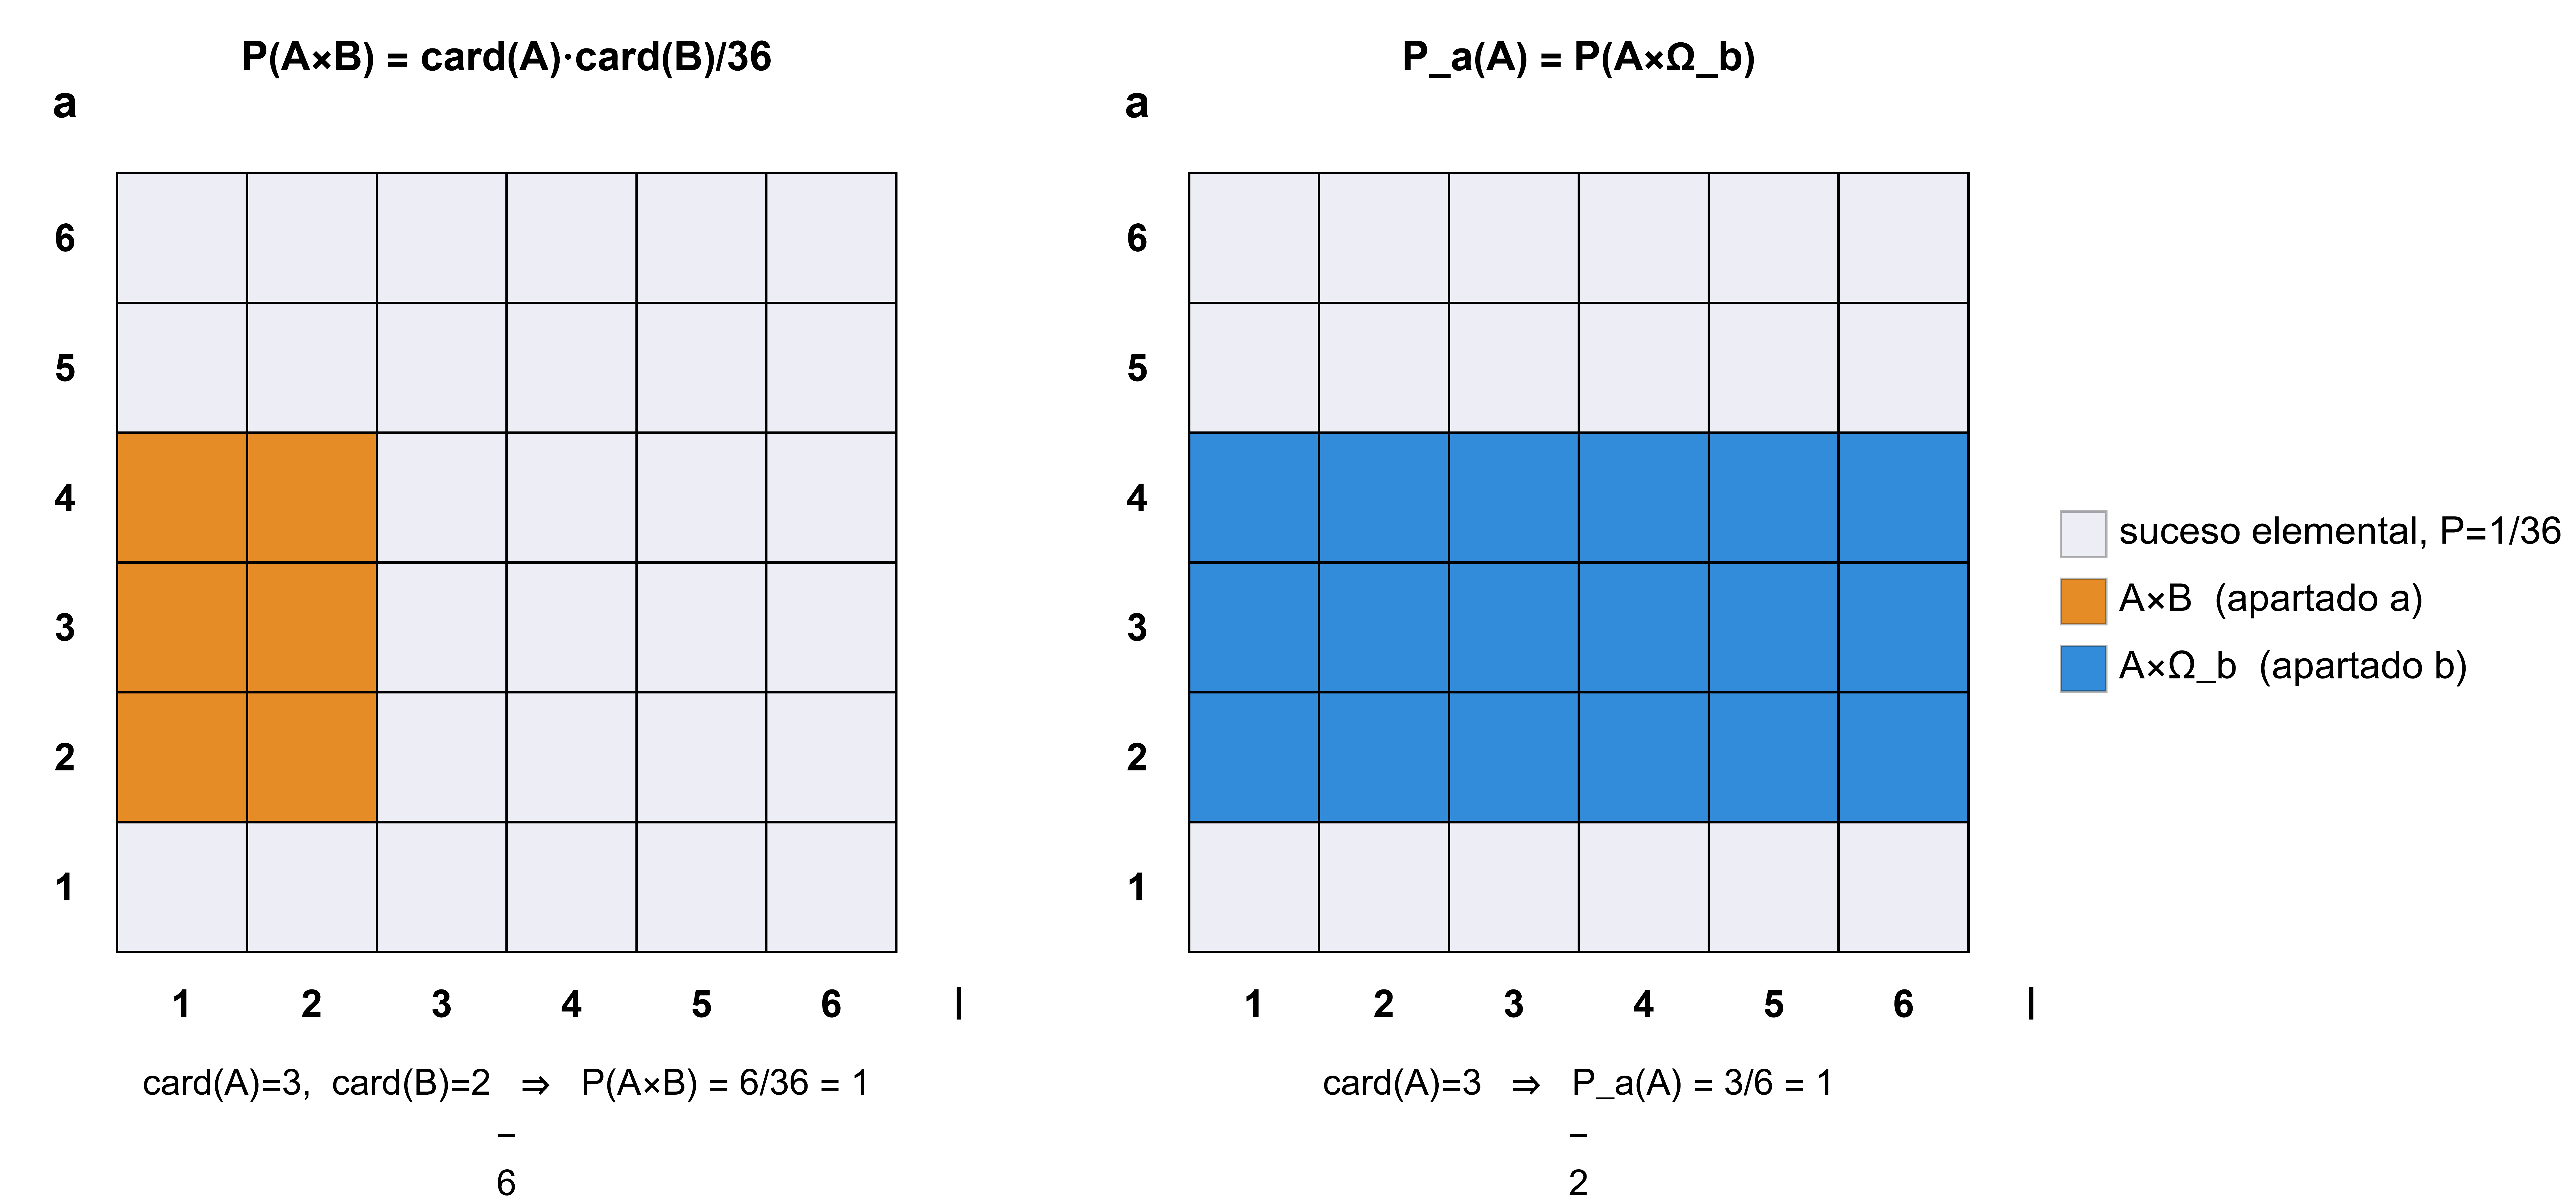
\includegraphics[width=1\linewidth]{imagenes/problemas_Quesada/prob_quesada_2_5_a}
\end{center}
\end{problema}

\newpage

% ------------------------------------------------------------------------------
% PROBLEMA 6
% ------------------------------------------------------------------------------
\begin{problema}[Límites superior e inferior de sucesiones de sucesos y de probabilidades]
Sea $\Omega = \{\omega_1, \omega_2, \omega_3, \omega_4\}$ y sea $P$ una medida de probabilidad definida sobre $\mathcal{P}(\Omega)$ tal que $P(\{\omega_1\}) = 1/6$, $P(\{\omega_2\}) = 1/3$, $P(\{\omega_3\}) = 1/5$ y $P(\{\omega_4\}) = 3/10$.

Dada la sucesión alternante de sucesos:
\[
    A_n = \begin{cases} \{\omega_1, \omega_2\} & \text{si } n \text{ es par} \\ \{\omega_2, \omega_3\} & \text{si } n \text{ es impar} \end{cases}
\]
Determinar $P(\varliminf_{n \to \infty} A_n)$, $\varliminf_{n \to \infty} P(A_n)$, $\varlimsup_{n \to \infty} P(A_n)$ y $P(\varlimsup_{n \to \infty} A_n)$.

\tcblower

\paragraph{1. Cálculo de los límites de conjuntos y sus probabilidades:}
El límite inferior $\varliminf_{n \to \infty} A_n$ consta de los elementos que pertenecen a todos los términos salvo a lo sumo un número finito, lo que para una sucesión periódica de periodo $2$ equivale a la intersección de sus términos distintos:
\[
    \varliminf_{n \to \infty} A_n = \{\omega_1, \omega_2\} \cap \{\omega_2, \omega_3\} = \{\omega_2\}
\]
Su probabilidad vale:
\[
    P\left( \varliminf_{n \to \infty} A_n \right) = P(\{\omega_2\}) = \frac{1}{3} = \frac{10}{30}
\]

El límite superior $\varlimsup_{n \to \infty} A_n$ consta de los elementos que pertenecen a infinitos términos de la sucesión, lo que equivale a la unión de sus términos distintos:
\[
    \varlimsup_{n \to \infty} A_n = \{\omega_1, \omega_2\} \cup \{\omega_2, \omega_3\} = \{\omega_1, \omega_2, \omega_3\}
\]
Por la aditividad de la probabilidad sobre sucesos disjuntos:
\[
    P\left( \varlimsup_{n \to \infty} A_n \right) = P(\{\omega_1\}) + P(\{\omega_2\}) + P(\{\omega_3\}) = \frac{1}{6} + \frac{1}{3} + \frac{1}{5} = \frac{7}{10} = \frac{21}{30}
\]
\vspace{0.5cm}
\begin{center}
    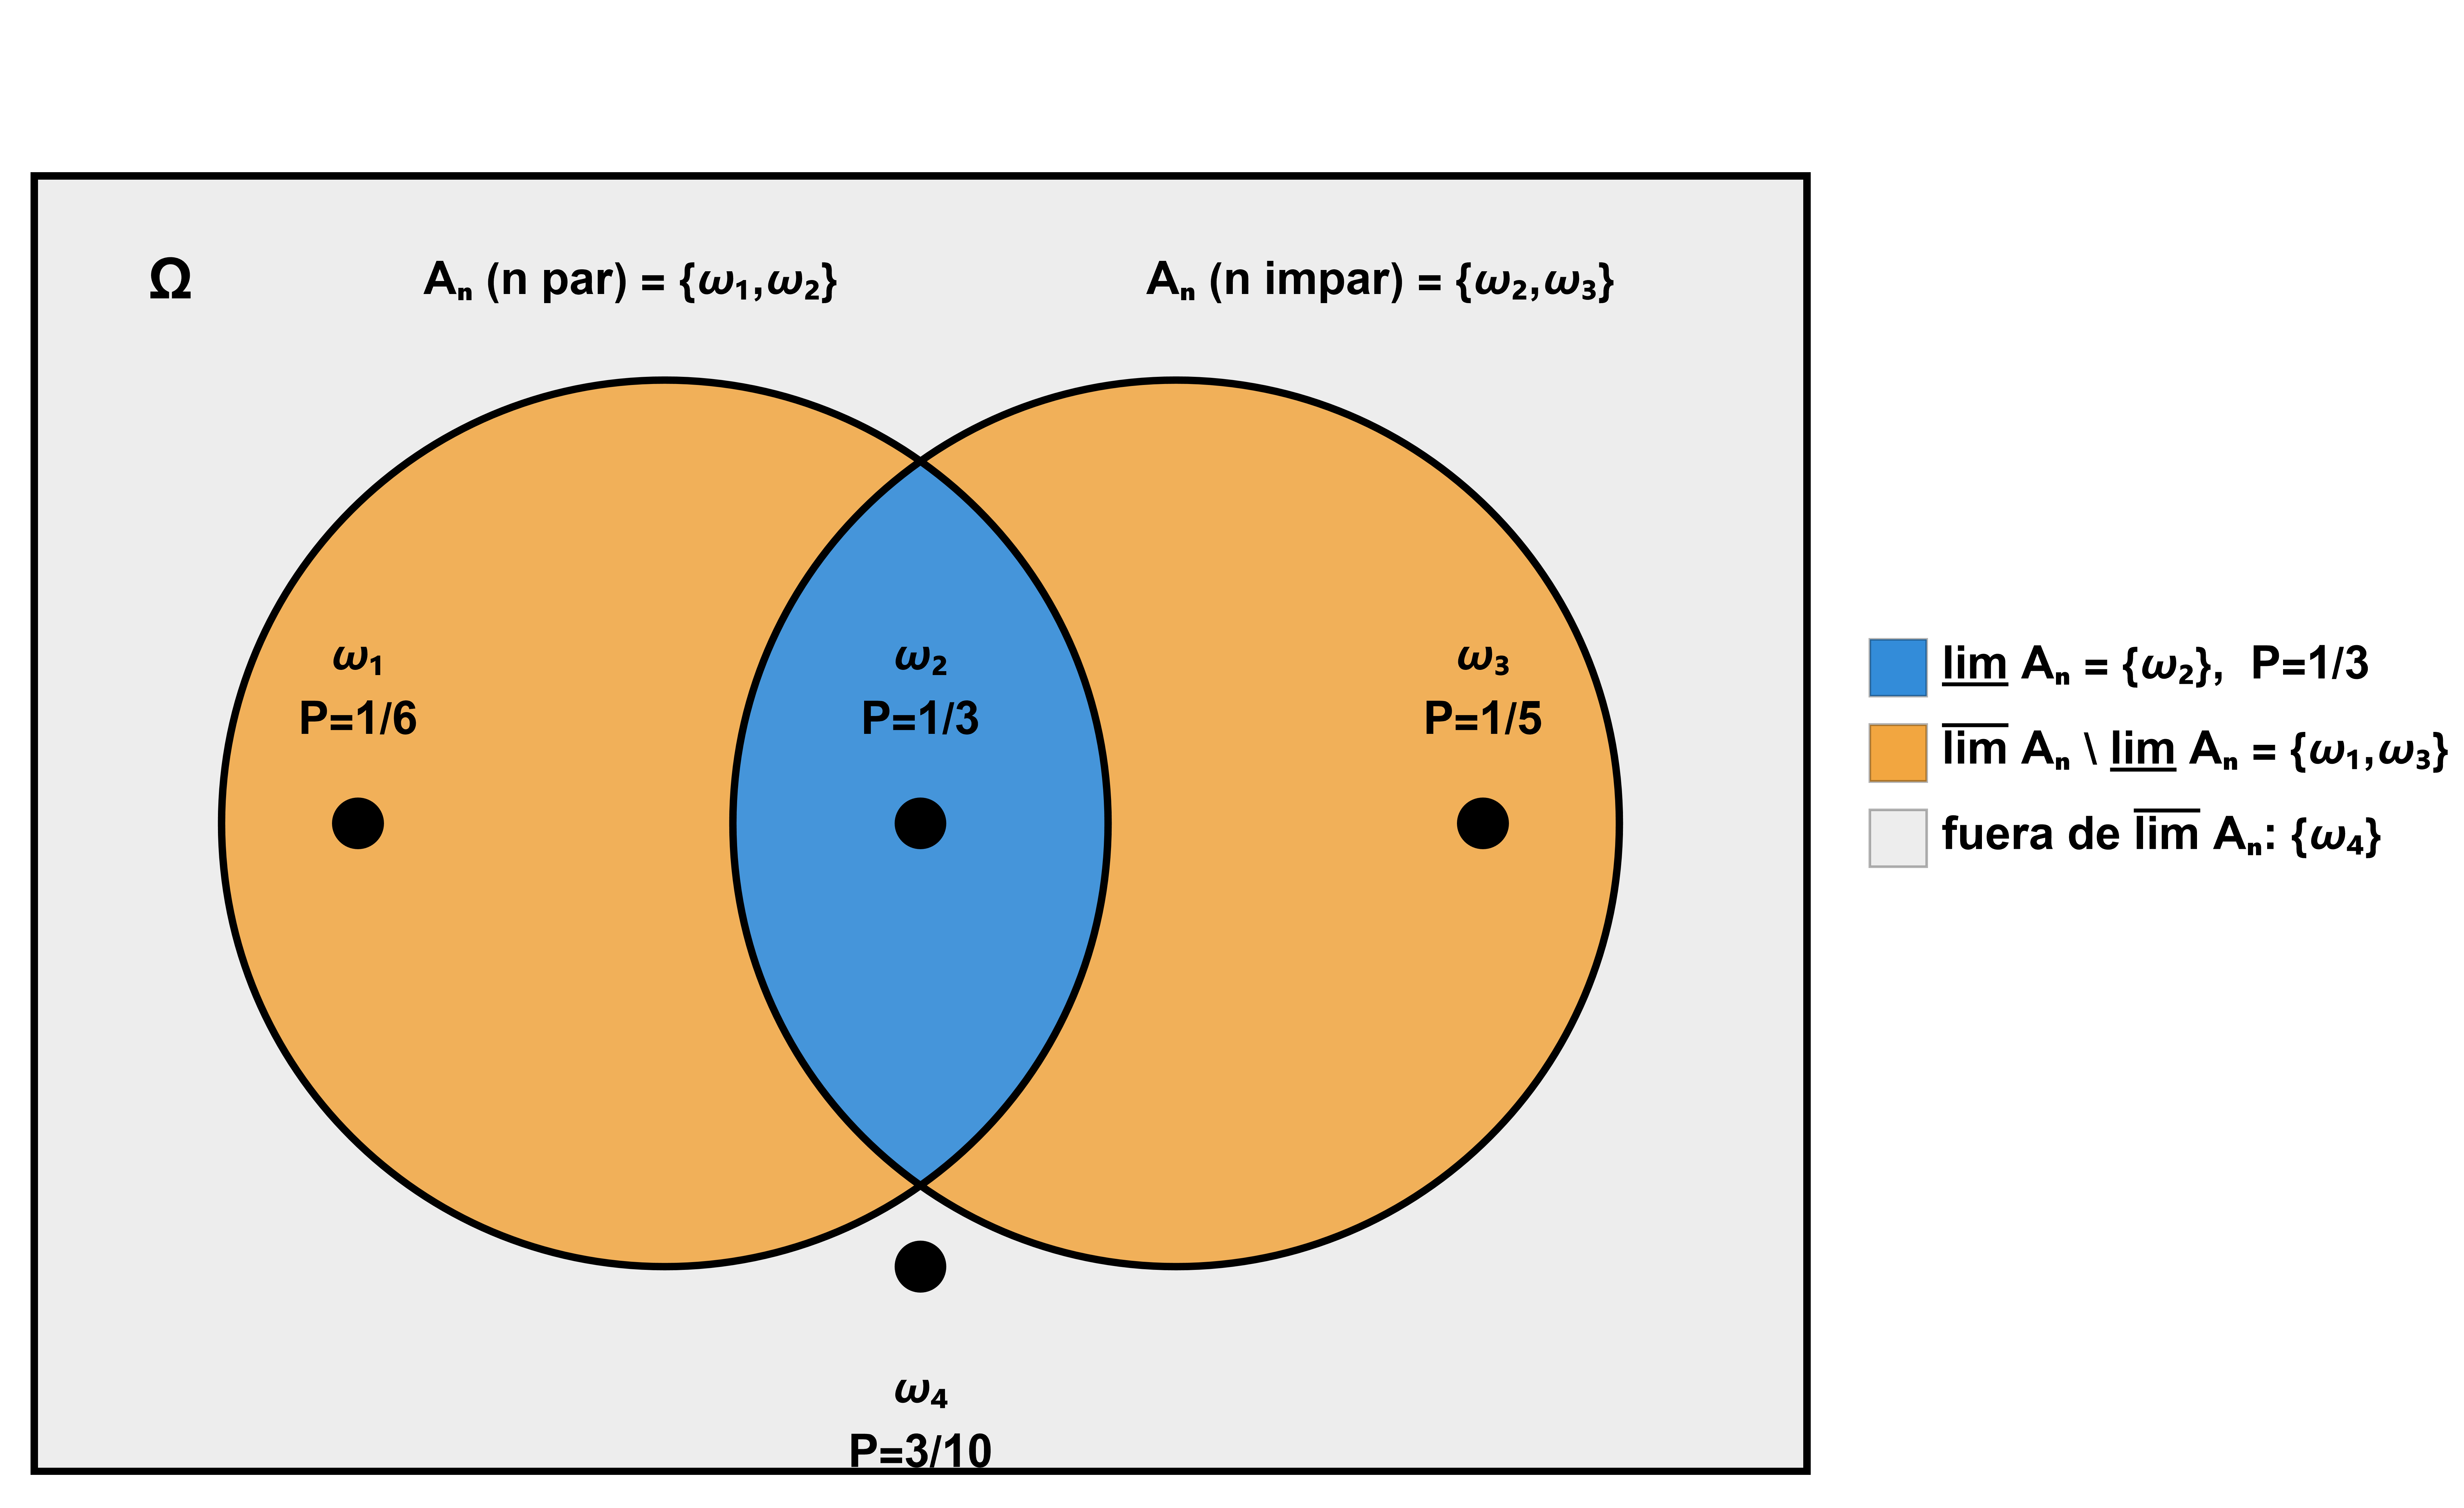
\includegraphics[width=0.8\linewidth]{imagenes/problemas_Quesada/prob_quesada_2_6_a}
\end{center}
\paragraph{2. Cálculo de la sucesión de probabilidades y sus límites numéricos:}
Evaluamos la probabilidad de $A_n$ según la paridad de $n$:
\[
    P(A_n) = \begin{cases}
        P(\{\omega_1, \omega_2\}) = \dfrac{1}{6} + \dfrac{1}{3} = \dfrac{1}{2} = \dfrac{15}{30} & \text{si } n \text{ es par} \\[0.5em]
        P(\{\omega_2, \omega_3\}) = \dfrac{1}{3} + \dfrac{1}{5} = \dfrac{8}{15} = \dfrac{16}{30} & \text{si } n \text{ es impar}
    \end{cases}
\]
Los límites inferior y superior de la sucesión numérica $P(A_n)$ vienen dados por el valor mínimo y máximo de sus subsucesiones convergentes:
\[
    \varliminf_{n \to \infty} P(A_n) = \min\left\{\frac{1}{2}, \frac{8}{15}\right\} = \frac{1}{2} = \frac{15}{30}
\]
\[
    \varlimsup_{n \to \infty} P(A_n) = \max\left\{\frac{1}{2}, \frac{8}{15}\right\} = \frac{8}{15} = \frac{16}{30}
\]

\paragraph{3. Comprobación del Teorema de continuidad para medidas (Corolario 1):}
Se comprueba que se satisface la cadena general de desigualdades para cualquier medida de probabilidad:
\[
    P\left( \varliminf_{n \to \infty} A_n \right) \le \varliminf_{n \to \infty} P(A_n) \le \varlimsup_{n \to \infty} P(A_n) \le P\left( \varlimsup_{n \to \infty} A_n \right)
\]
Sustituyendo los valores obtenidos expresados en un denominador común:
\[
    \frac{10}{30} < \frac{15}{30} < \frac{16}{30} < \frac{21}{30} \implies \frac{1}{3} < \frac{1}{2} < \frac{8}{15} < \frac{7}{10}
\]
En este caso particular, todas las desigualdades resultan ser estrictas.
\end{problema}

\newpage

% ------------------------------------------------------------------------------
% PROBLEMA 7
% ------------------------------------------------------------------------------
\begin{problema}[Probabilidades en una $\sigma$-álgebra generada por dos conjuntos]
Considérese el espacio muestral $\Omega = \{\omega_1, \omega_2, \omega_3, \omega_4\}$, la $\sigma$-álgebra de subconjuntos de $\Omega$ generada por los conjuntos $A = \{\omega_1, \omega_2\}$ y $B = \{\omega_2, \omega_3, \omega_4\}$, y la medida de probabilidad sobre el espacio probabilizable $(\Omega, \mathcal{Q})$ tal que $P(\{\omega_1\}) = P(\{\omega_2\}) = \frac{P(B)}{2}$. Se pide:
\begin{enumerate}[label=\alph*)]
    \item Determinar las probabilidades de los cuatro puntos muestrales.
    \item Calcular $P(A)$ y $P(\{\omega_3, \omega_4\})$.
\end{enumerate}

\tcblower

\paragraph{1. Determinación de la $\sigma$-álgebra generada $\mathcal{Q} = \sigma(A, B)$:}
Partimos de la colección generadora $\mathcal{C} = \{A, B\}$. Los átomos (sucesos elementales medibles minimales) se obtienen mediante las intersecciones no vacías de $A, A^c$ y $B, B^c$:
\begin{itemize}
    \item $A \cap B = \{\omega_2\}$
    \item $A \cap B^c = \{\omega_1\}$
    \item $A^c \cap B = \{\omega_3, \omega_4\}$
    \item $A^c \cap B^c = \varnothing$
\end{itemize}
La $\sigma$-álgebra generada $\mathcal{Q} = \sigma(\mathcal{C})$ está formada por todas las uniones posibles de estos tres átomos disjuntos $\{\omega_1\}$, $\{\omega_2\}$ y $\{\omega_3, \omega_4\}$, constando de $2^3 = 8$ elementos:
\[
    \mathcal{Q} = \bigl\{ \varnothing, \, \{\omega_1\}, \, \{\omega_2\}, \, \{\omega_3, \omega_4\}, \, \{\omega_1, \omega_2\}, \, \{\omega_1, \omega_3, \omega_4\}, \, \{\omega_2, \omega_3, \omega_4\}, \, \Omega \bigr\}
\]
Observamos que los subconjuntos unipuntuales $\{\omega_3\}$ y $\{\omega_4\}$ no pertenecen a $\mathcal{Q}$, por lo que no constituyen sucesos medibles.

\paragraph{a) Probabilidades de los puntos muestrales:}
Puesto que $B = \{\omega_2, \omega_3, \omega_4\} = \{\omega_2\} \sqcup \{\omega_3, \omega_4\}$ y $\{\omega_1\} \sqcup B = \Omega$, los sucesos $\{\omega_1\}$ y $B$ constituyen una partición del espacio universal $\Omega$. Por el axioma de normalización y la aditividad finita:
\[
    P(\{\omega_1\}) + P(B) = P(\Omega) = 1
\]
Sustituyendo la condición $P(B) = 2 P(\{\omega_1\})$:
\[
    P(\{\omega_1\}) + 2 P(\{\omega_1\}) = 1 \implies 3 P(\{\omega_1\}) = 1 \implies P(\{\omega_1\}) = \frac{1}{3}
\]
Por consiguiente, deducimos:
\[
    P(\{\omega_1\}) = \frac{1}{3}, \quad P(\{\omega_2\}) = \frac{1}{3}, \quad P(B) = \frac{2}{3}
\]
Por otro lado, dado que $\{\omega_3\} \notin \mathcal{Q}$ y $\{\omega_4\} \notin \mathcal{Q}$, las probabilidades individuales de $\omega_3$ y $\omega_4$ no están definidas dentro del espacio probabilístico $(\Omega, \mathcal{Q}, P)$.

\paragraph{b) Cálculo de $P(A)$ y $P(\{\omega_3, \omega_4\})$:}
\begin{itemize}
    \item Puesto que $A = \{\omega_1, \omega_2\} = \{\omega_1\} \sqcup \{\omega_2\}$, por la aditividad de la medida de probabilidad:
    \[
        P(A) = P(\{\omega_1\}) + P(\{\omega_2\}) = \frac{1}{3} + \frac{1}{3} = \frac{2}{3}
    \]
    \item El suceso $\{\omega_3, \omega_4\}$ es el complementario de $A$ respecto a $\Omega$, es decir, $\{\omega_3, \omega_4\} = A^c \in \mathcal{Q}$. Por la propiedad del suceso contrario:
    \[
        P(\{\omega_3, \omega_4\}) = P(A^c) = 1 - P(A) = 1 - \frac{2}{3} = \frac{1}{3}
    \]
\end{itemize}

\vspace{0.5cm}
\begin{center}
    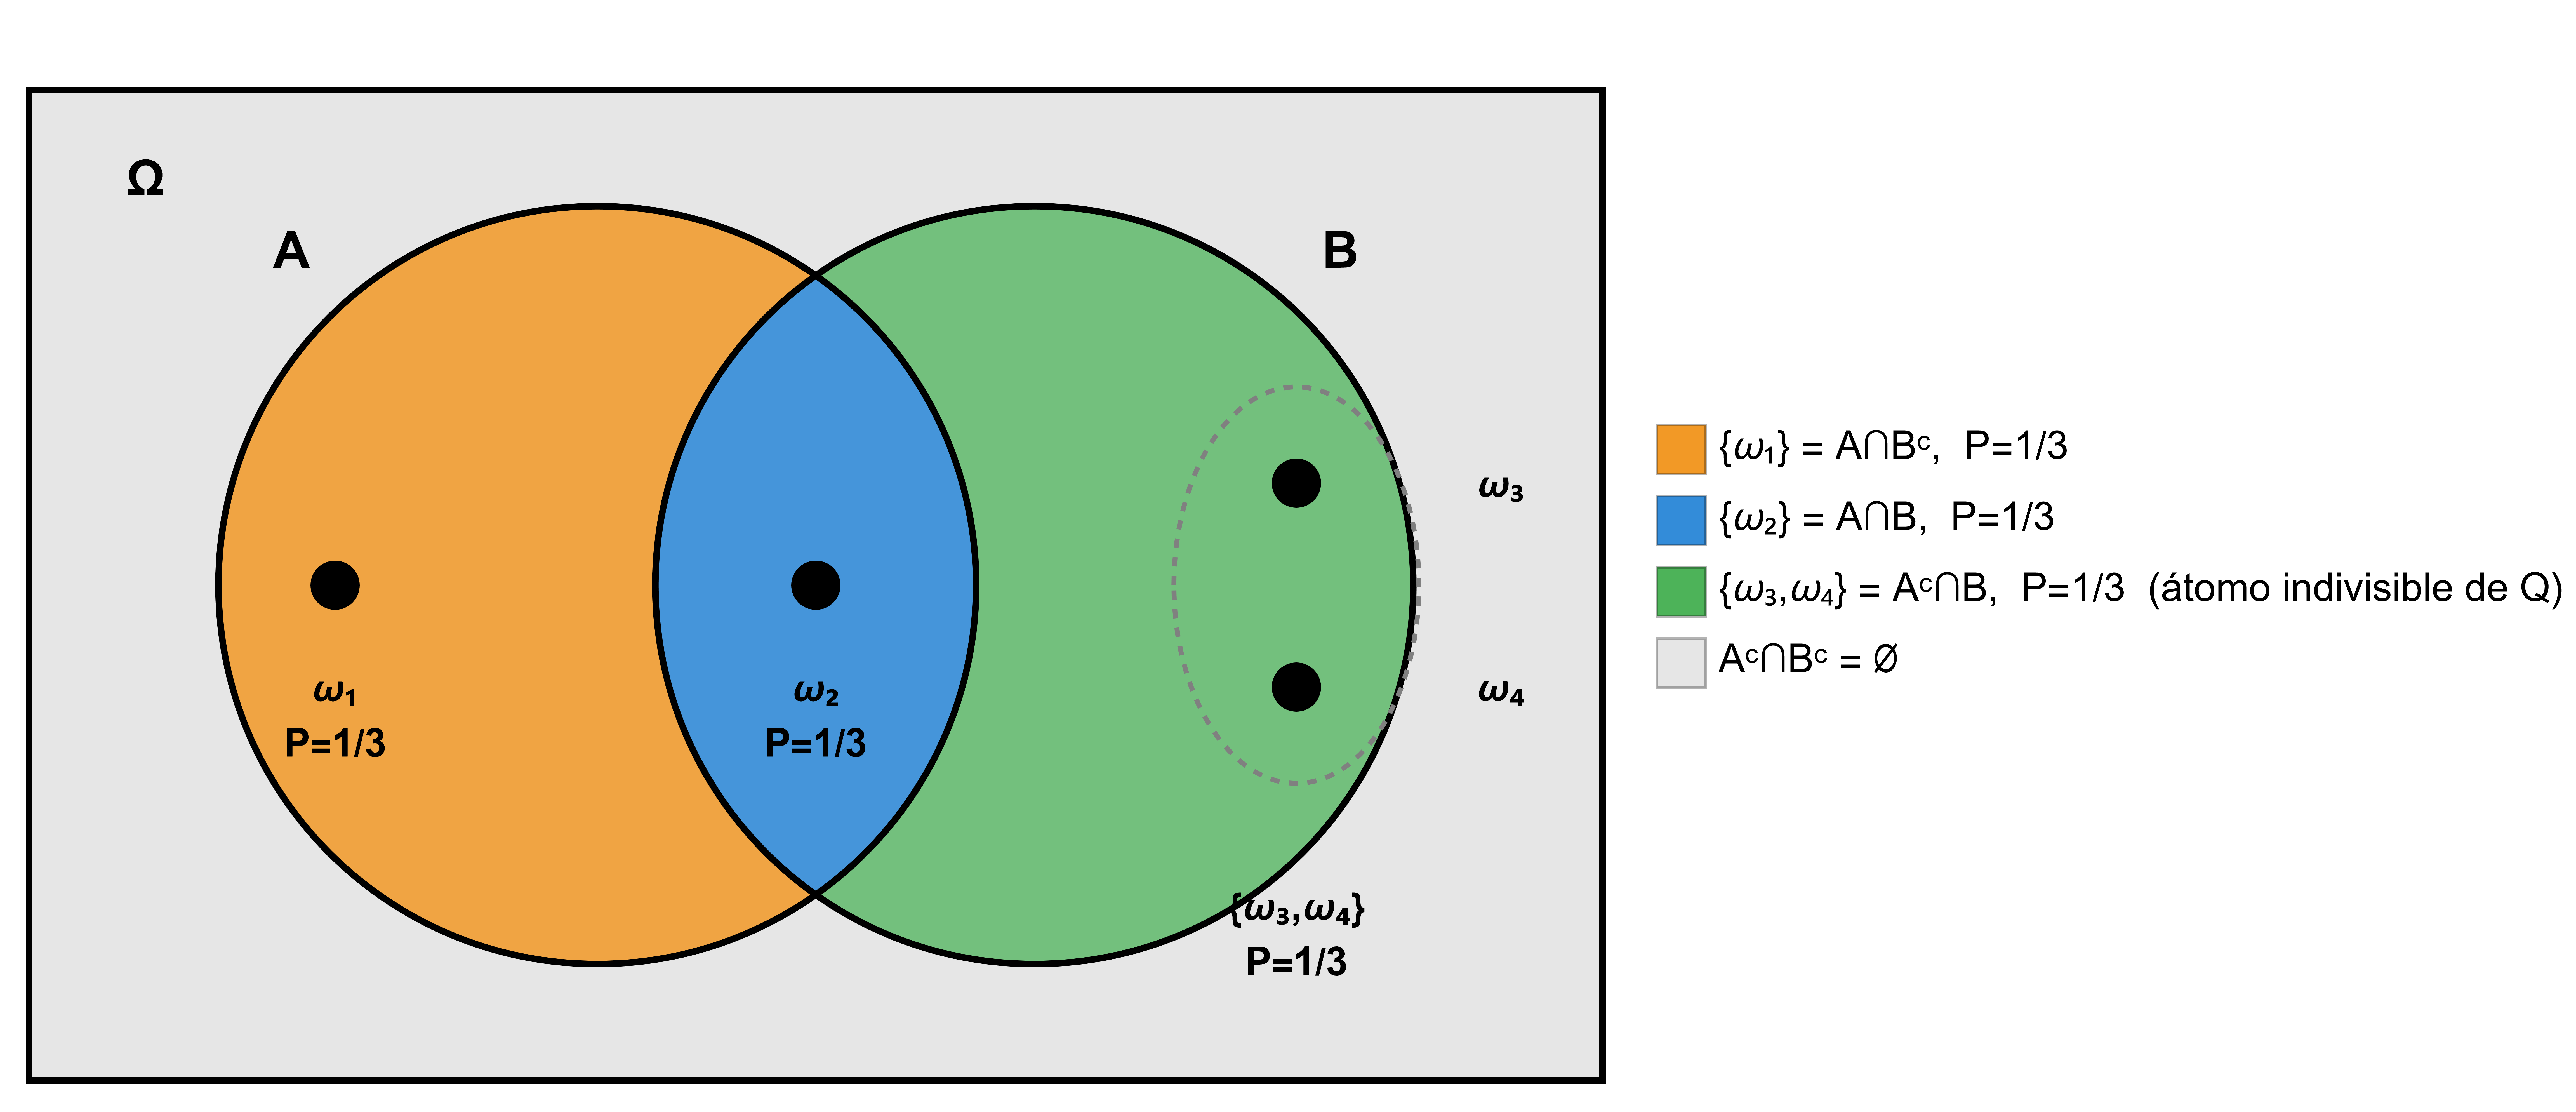
\includegraphics[width=1\linewidth]{imagenes/problemas_Quesada/prob_quesada_2_7_a}
\end{center}
\end{problema}

\newpage
% ------------------------------------------------------------------------------
% PROBLEMA 8
% ------------------------------------------------------------------------------
\begin{problema}[Cálculo de probabilidades para tres sucesos]
Sean $A, B$ y $C$ tres sucesos de un espacio probabilístico $(\Omega, \mathcal{Q}, P)$ tales que $P(A) = 0.4$, $P(B) = 0.2$, $P(C) = 0.3$, $P(A \cap B) = 0.1$ y $(A \cup B) \cap C = \varnothing$. Calcular las probabilidades de los siguientes sucesos:
\begin{enumerate}[label=\alph*)]
    \item Solamente ocurre $A$.
    \item Los tres sucesos ocurren.
    \item Ocurren $A$ y $B$, pero no $C$.
    \item Por lo menos dos ocurren.
    \item Ocurren dos y no más.
    \item No ocurren más de dos.
    \item Ocurre por lo menos uno.
    \item Ocurre sólo uno.
    \item No ocurre ninguno.
\end{enumerate}

\tcblower

\paragraph{Análisis previo de la condición de disjuntismo:}
La condición $(A \cup B) \cap C = \varnothing$ establece que $C$ es disjunto con la unión $A \cup B$. Por la propiedad distributiva de la intersección:
\[
    (A \cap C) \cup (B \cap C) = \varnothing \implies A \cap C = \varnothing \quad \text{y} \quad B \cap C = \varnothing
\]
En particular, las probabilidades asociadas a estas intersecciones se anulan:
\[
    P(A \cap C) = 0, \quad P(B \cap C) = 0, \quad P(A \cap B \cap C) = 0
\]

\paragraph{a) Solamente ocurre $A$ ($A \cap B^c \cap C^c$):}
Al ser $A \cap C = \varnothing$, se cumple $A \subseteq C^c$, por lo que $A \cap C^c = A$. El suceso se reduce a $A \setminus B$:
\[
    P(A \cap B^c \cap C^c) = P(A \setminus B) = P(A) - P(A \cap B) = 0.4 - 0.1 = 0.3
\]

\paragraph{b) Los tres sucesos ocurren ($A \cap B \cap C$):}
Como $A \cap B \cap C \subseteq (A \cup B) \cap C = \varnothing$:
\[
    P(A \cap B \cap C) = P(\varnothing) = 0
\]

\paragraph{c) Ocurren $A$ y $B$, pero no $C$ ($A \cap B \cap C^c$):}
Al ser $A \cap B \subseteq A \cup B$ y $(A \cup B) \cap C = \varnothing$, el suceso $A \cap B$ está completamente contenido en $C^c$:
\[
    P(A \cap B \cap C^c) = P(A \cap B) = 0.1
\]

\paragraph{d) Por lo menos dos ocurren:}
Expresamos el suceso mediante la unión de las tres posibles intersecciones dobles:
\[
    (A \cap B) \cup (A \cap C) \cup (B \cap C) = (A \cap B) \cup \varnothing \cup \varnothing = A \cap B
\]
\[
    P(\text{por lo menos dos}) = P(A \cap B) = 0.1
\]

\paragraph{e) Ocurren dos y no más (exactamente dos):}
Equivale a que ocurran por lo menos dos pero no los tres simultáneamente:
\[
    P(\text{exactamente dos}) = P(\text{por lo menos dos}) - P(A \cap B \cap C) = 0.1 - 0 = 0.1
\]

\paragraph{f) No ocurren más de dos:}
Es el suceso contrario a que ocurran los tres sucesos a la vez:
\[
    P(\text{no ocurren más de dos}) = 1 - P(A \cap B \cap C) = 1 - 0 = 1
\]

\paragraph{g) Ocurre por lo menos uno ($A \cup B \cup C$):}
Dado que $C$ es disjunto con $A \cup B$:
\[
    P(A \cup B \cup C) = P(A \cup B) + P(C)
\]
Calculamos primero $P(A \cup B)$:
\[
    P(A \cup B) = P(A) + P(B) - P(A \cap B) = 0.4 + 0.2 - 0.1 = 0.5
\]
Sustituyendo obtenemos:
\[
    P(A \cup B \cup C) = 0.5 + 0.3 = 0.8
\]

\paragraph{h) Ocurre sólo uno (exactamente uno):}
Es la diferencia entre que ocurra por lo menos uno y que ocurran por lo menos dos:
\[
    P(\text{exactamente uno}) = P(A \cup B \cup C) - P(\text{por lo menos dos}) = 0.8 - 0.1 = 0.7
\]
\textit{Demostración alternativa:} Sumamos las probabilidades de la ocurrencia exclusiva de cada suceso:
\[
    P(A \setminus B) + P(B \setminus A) + P(C) = (0.4 - 0.1) + (0.2 - 0.1) + 0.3 = 0.3 + 0.1 + 0.3 = 0.7
\]

\paragraph{i) No ocurre ninguno ($(A \cup B \cup C)^c$):}
Es el suceso contrario a que ocurra al menos uno:
\[
    P\bigl((A \cup B \cup C)^c\bigr) = 1 - P(A \cup B \cup C) = 1 - 0.8 = 0.2
\]

\vspace{0.5cm}
\begin{center}
    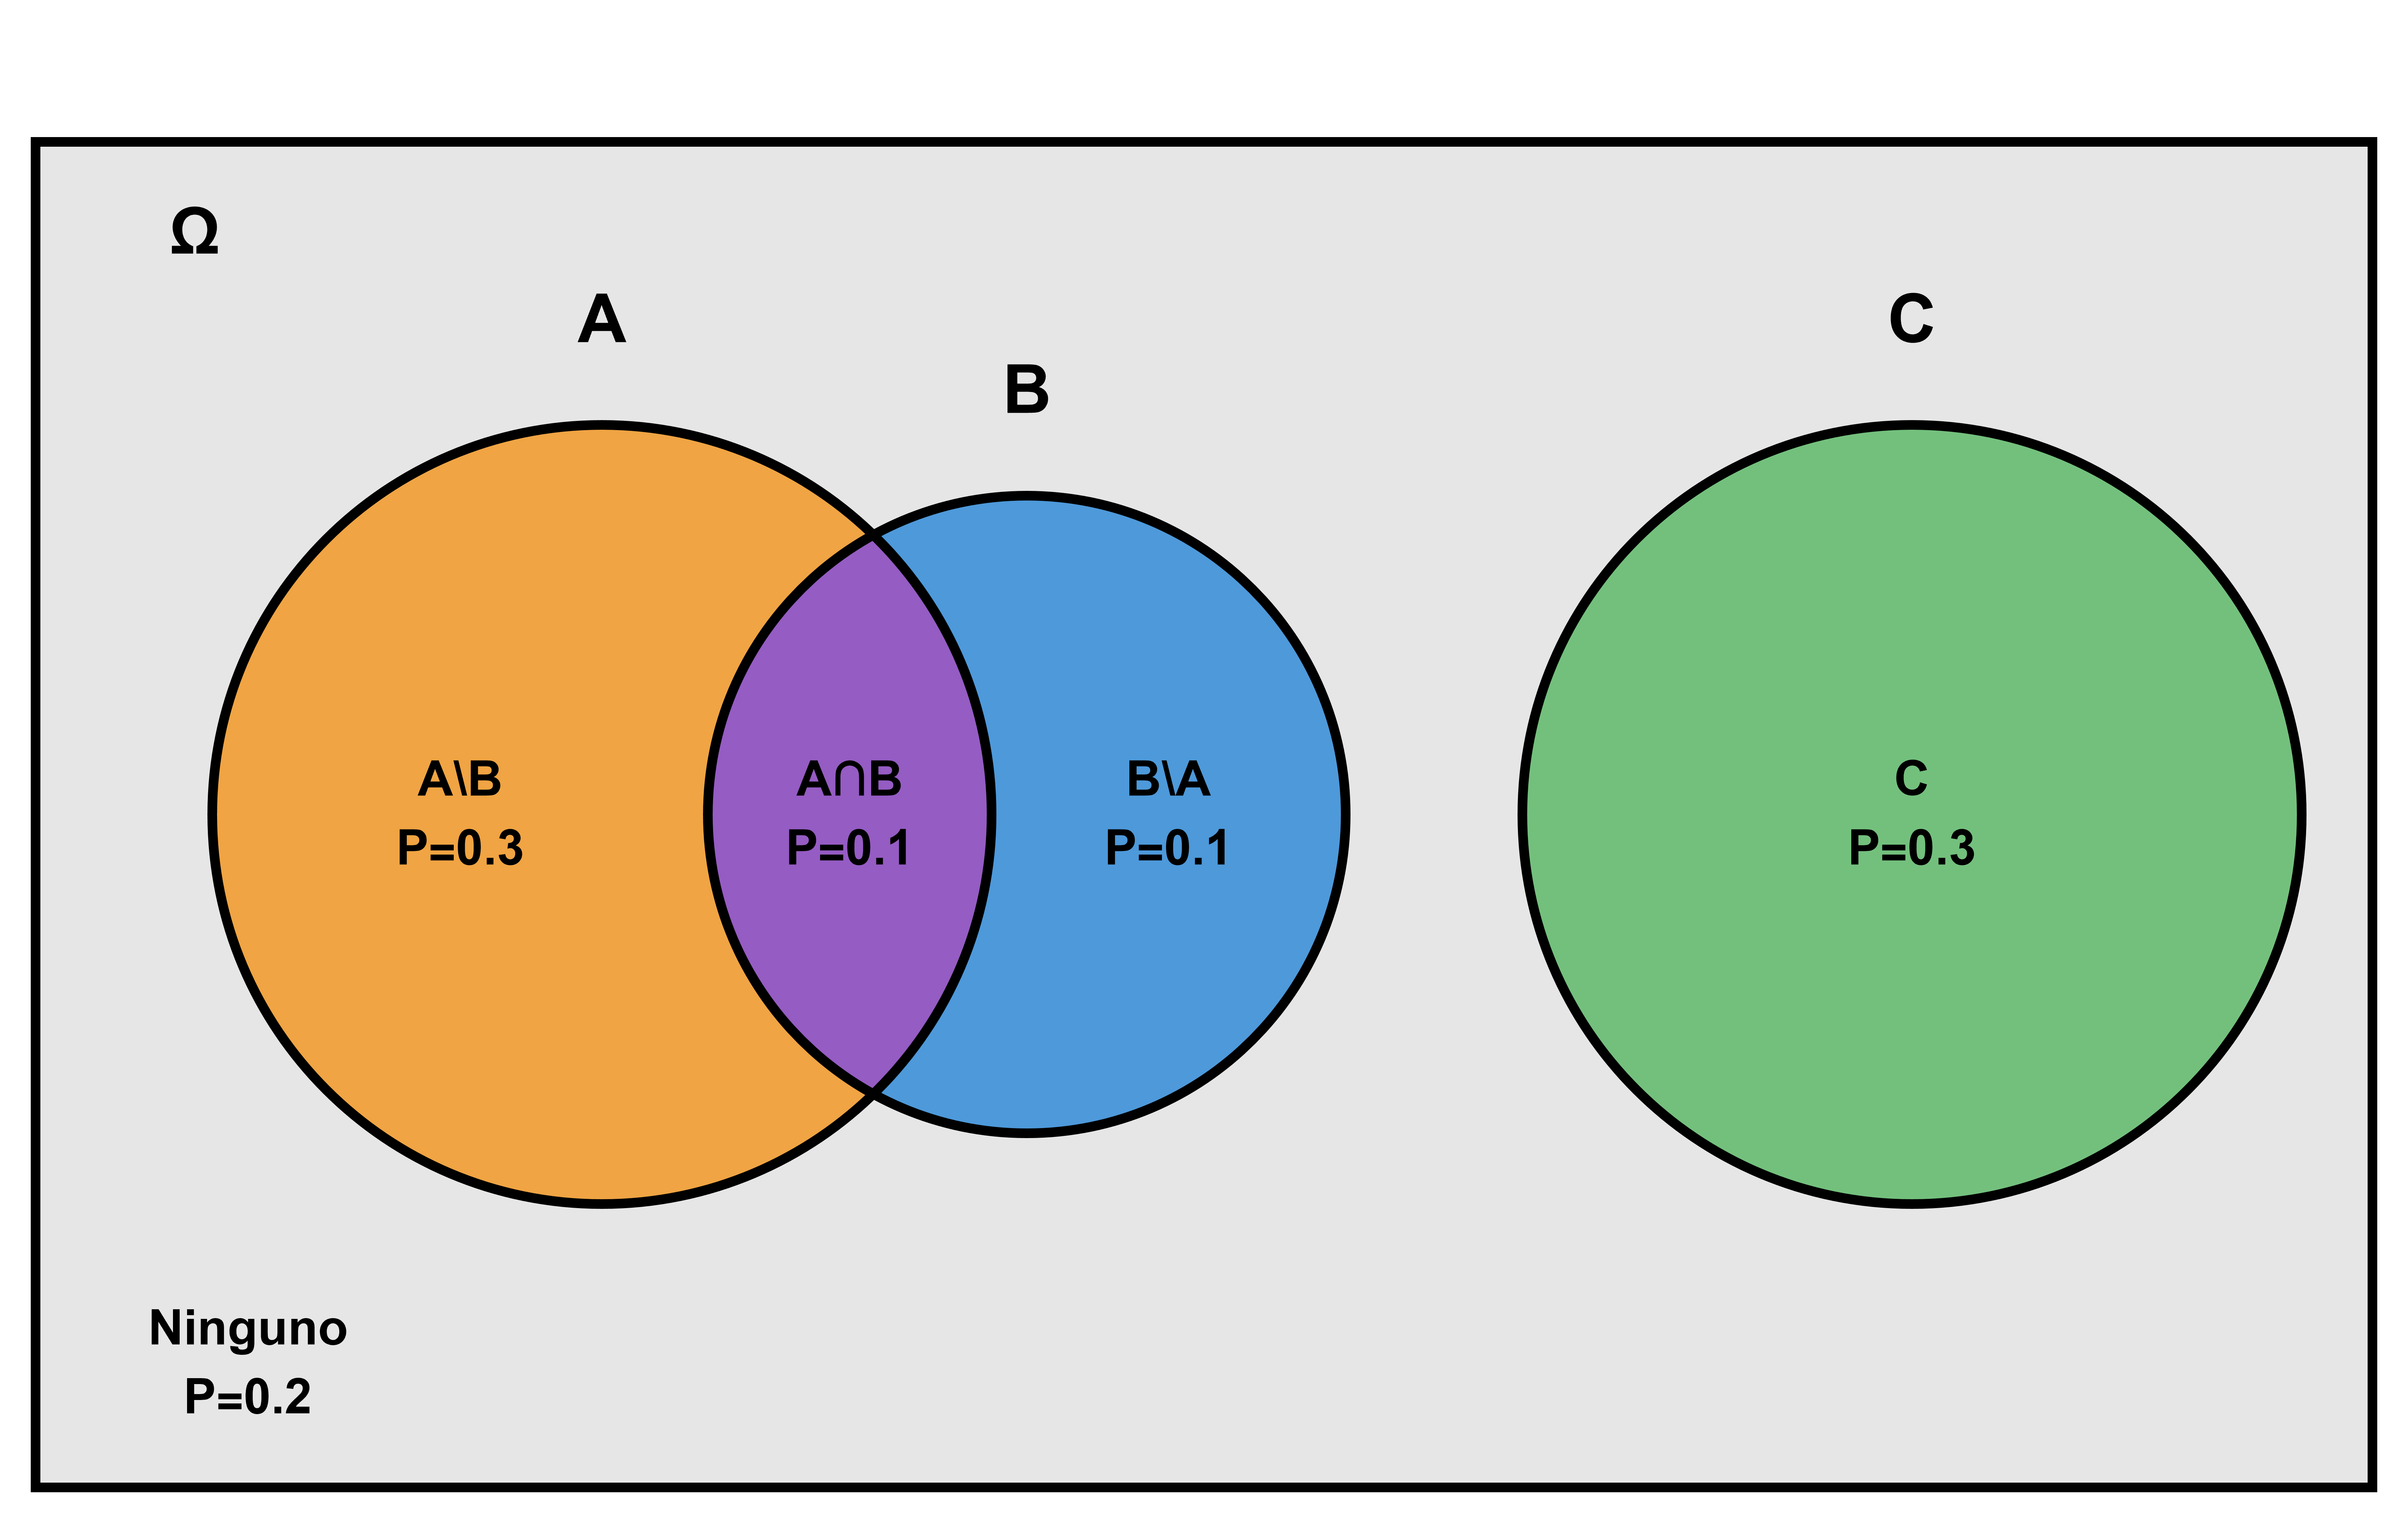
\includegraphics[width=1\linewidth]{imagenes/problemas_Quesada/prob_quesada_2_8_a}
\end{center}
\end{problema}